
%% bare_conf.tex
%% V1.3
%% 2007/01/11
%% by Michael Shell
%% See:
%% http://www.michaelshell.org/
%% for current contact information.
%%
%% This is a skeleton file demonstrating the use of IEEEtran.cls
%% (requires IEEEtran.cls version 1.7 or later) with an IEEE conference paper.
%%
%% Support sites:
%% http://www.michaelshell.org/tex/ieeetran/
%% http://www.ctan.org/tex-archive/macros/latex/contrib/IEEEtran/
%% and
%% http://www.ieee.org/

%%*************************************************************************
%% Legal Notice:
%% This code is offered as-is without any warranty either expressed or
%% implied; without even the implied warranty of MERCHANTABILITY or
%% FITNESS FOR A PARTICULAR PURPOSE! 
%% User assumes all risk.
%% In no event shall IEEE or any contributor to this code be liable for
%% any damages or losses, including, but not limited to, incidental,
%% consequential, or any other damages, resulting from the use or misuse
%% of any information contained here.
%%
%% All comments are the opinions of their respective authors and are not
%% necessarily endorsed by the IEEE.
%%
%% This work is distributed under the LaTeX Project Public License (LPPL)
%% ( http://www.latex-project.org/ ) version 1.3, and may be freely used,
%% distributed and modified. A copy of the LPPL, version 1.3, is included
%% in the base LaTeX documentation of all distributions of LaTeX released
%% 2003/12/01 or later.
%% Retain all contribution notices and credits.
%% ** Modified files should be clearly indicated as such, including  **
%% ** renaming them and changing author support contact information. **
%%
%% File list of work: IEEEtran.cls, IEEEtran_HOWTO.pdf, bare_adv.tex,
%%                    bare_conf.tex, bare_jrnl.tex, bare_jrnl_compsoc.tex
%%*************************************************************************

% *** Authors should verify (and, if needed, correct) their LaTeX system  ***
% *** with the testflow diagnostic prior to trusting their LaTeX platform ***
% *** with production work. IEEE's font choices can trigger bugs that do  ***
% *** not appear when using other class files.                            ***
% The testflow support page is at:
% http://www.michaelshell.org/tex/testflow/



% Note that the a4paper option is mainly intended so that authors in
% countries using A4 can easily print to A4 and see how their papers will
% look in print - the typesetting of the document will not typically be
% affected with changes in paper size (but the bottom and side margins will).
% Use the testflow package mentioned above to verify correct handling of
% both paper sizes by the user's LaTeX system.
%
% Also note that the "draftcls" or "draftclsnofoot", not "draft", option
% should be used if it is desired that the figures are to be displayed in
% draft mode.
%
%\documentclass[conference, letterpaper]{./IEEEtran}
\documentclass[peerreviewca, letterpaper]{./IEEEtran}
% Add the compsoc option for Computer Society conferences.
%
% If IEEEtran.cls has not been installed into the LaTeX system files,
% manually specify the path to it like:
% \documentclass[conference]{../sty/IEEEtran}

\usepackage[latin9]{inputenc}




% Some very useful LaTeX packages include:
% (uncomment the ones you want to load)


% *** MISC UTILITY PACKAGES ***
%
%\usepackage{ifpdf}
% Heiko Oberdiek's ifpdf.sty is very useful if you need conditional
% compilation based on whether the output is pdf or dvi.
% usage:
% \ifpdf
%   % pdf code
% \else
%   % dvi code
% \fi
% The latest version of ifpdf.sty can be obtained from:
% http://www.ctan.org/tex-archive/macros/latex/contrib/oberdiek/
% Also, note that IEEEtran.cls V1.7 and later provides a builtin
% \ifCLASSINFOpdf conditional that works the same way.
% When switching from latex to pdflatex and vice-versa, the compiler may
% have to be run twice to clear warning/error messages.






% *** CITATION PACKAGES ***
%
%\usepackage{cite}
% cite.sty was written by Donald Arseneau
% V1.6 and later of IEEEtran pre-defines the format of the cite.sty package
% \cite{} output to follow that of IEEE. Loading the cite package will
% result in citation numbers being automatically sorted and properly
% "compressed/ranged". e.g., [1], [9], [2], [7], [5], [6] without using
% cite.sty will become [1], [2], [5]--[7], [9] using cite.sty. cite.sty's
% \cite will automatically add leading space, if needed. Use cite.sty's
% noadjust option (cite.sty V3.8 and later) if you want to turn this off.
% cite.sty is already installed on most LaTeX systems. Be sure and use
% version 4.0 (2003-05-27) and later if using hyperref.sty. cite.sty does
% not currently provide for hyperlinked citations.
% The latest version can be obtained at:
% http://www.ctan.org/tex-archive/macros/latex/contrib/cite/
% The documentation is contained in the cite.sty file itself.






% *** GRAPHICS RELATED PACKAGES ***
%
\ifCLASSINFOpdf
  % \usepackage[pdftex]{graphicx}
  % declare the path(s) where your graphic files are
  % \graphicspath{{../pdf/}{../jpeg/}}
  % and their extensions so you won't have to specify these with
  % every instance of \includegraphics
  % \DeclareGraphicsExtensions{.pdf,.jpeg,.png}
\else
  % or other class option (dvipsone, dvipdf, if not using dvips). graphicx
  % will default to the driver specified in the system graphics.cfg if no
  % driver is specified.
  % \usepackage[dvips]{graphicx}
  % declare the path(s) where your graphic files are
  % \graphicspath{{../eps/}}
  % and their extensions so you won't have to specify these with
  % every instance of \includegraphics
  % \DeclareGraphicsExtensions{.eps}
\fi
% graphicx was written by David Carlisle and Sebastian Rahtz. It is
% required if you want graphics, photos, etc. graphicx.sty is already
% installed on most LaTeX systems. The latest version and documentation can
% be obtained at: 
% http://www.ctan.org/tex-archive/macros/latex/required/graphics/
% Another good source of documentation is "Using Imported Graphics in
% LaTeX2e" by Keith Reckdahl which can be found as epslatex.ps or
% epslatex.pdf at: http://www.ctan.org/tex-archive/info/
%
% latex, and pdflatex in dvi mode, support graphics in encapsulated
% postscript (.eps) format. pdflatex in pdf mode supports graphics
% in .pdf, .jpeg, .png and .mps (metapost) formats. Users should ensure
% that all non-photo figures use a vector format (.eps, .pdf, .mps) and
% not a bitmapped formats (.jpeg, .png). IEEE frowns on bitmapped formats
% which can result in "jaggedy"/blurry rendering of lines and letters as
% well as large increases in file sizes.
%
% You can find documentation about the pdfTeX application at:
% http://www.tug.org/applications/pdftex





% *** MATH PACKAGES ***
%
%\usepackage[cmex10]{amsmath}
% A popular package from the American Mathematical Society that provides
% many useful and powerful commands for dealing with mathematics. If using
% it, be sure to load this package with the cmex10 option to ensure that
% only type 1 fonts will utilized at all point sizes. Without this option,
% it is possible that some math symbols, particularly those within
% footnotes, will be rendered in bitmap form which will result in a
% document that can not be IEEE Xplore compliant!
%
% Also, note that the amsmath package sets \interdisplaylinepenalty to 10000
% thus preventing page breaks from occurring within multiline equations. Use:
%\interdisplaylinepenalty=2500
% after loading amsmath to restore such page breaks as IEEEtran.cls normally
% does. amsmath.sty is already installed on most LaTeX systems. The latest
% version and documentation can be obtained at:
% http://www.ctan.org/tex-archive/macros/latex/required/amslatex/math/





% *** SPECIALIZED LIST PACKAGES ***
%
%\usepackage{algorithmic}
% algorithmic.sty was written by Peter Williams and Rogerio Brito.
% This package provides an algorithmic environment fo describing algorithms.
% You can use the algorithmic environment in-text or within a figure
% environment to provide for a floating algorithm. Do NOT use the algorithm
% floating environment provided by algorithm.sty (by the same authors) or
% algorithm2e.sty (by Christophe Fiorio) as IEEE does not use dedicated
% algorithm float types and packages that provide these will not provide
% correct IEEE style captions. The latest version and documentation of
% algorithmic.sty can be obtained at:
% http://www.ctan.org/tex-archive/macros/latex/contrib/algorithms/
% There is also a support site at:
% http://algorithms.berlios.de/index.html
% Also of interest may be the (relatively newer and more customizable)
% algorithmicx.sty package by Szasz Janos:
% http://www.ctan.org/tex-archive/macros/latex/contrib/algorithmicx/




% *** ALIGNMENT PACKAGES ***
%
%\usepackage{array}
% Frank Mittelbach's and David Carlisle's array.sty patches and improves
% the standard LaTeX2e array and tabular environments to provide better
% appearance and additional user controls. As the default LaTeX2e table
% generation code is lacking to the point of almost being broken with
% respect to the quality of the end results, all users are strongly
% advised to use an enhanced (at the very least that provided by array.sty)
% set of table tools. array.sty is already installed on most systems. The
% latest version and documentation can be obtained at:
% http://www.ctan.org/tex-archive/macros/latex/required/tools/


%\usepackage{mdwmath}
%\usepackage{mdwtab}
% Also highly recommended is Mark Wooding's extremely powerful MDW tools,
% especially mdwmath.sty and mdwtab.sty which are used to format equations
% and tables, respectively. The MDWtools set is already installed on most
% LaTeX systems. The lastest version and documentation is available at:
% http://www.ctan.org/tex-archive/macros/latex/contrib/mdwtools/


% IEEEtran contains the IEEEeqnarray family of commands that can be used to
% generate multiline equations as well as matrices, tables, etc., of high
% quality.


%\usepackage{eqparbox}
% Also of notable interest is Scott Pakin's eqparbox package for creating
% (automatically sized) equal width boxes - aka "natural width parboxes".
% Available at:
% http://www.ctan.org/tex-archive/macros/latex/contrib/eqparbox/





% *** SUBFIGURE PACKAGES ***
%\usepackage[tight,footnotesize]{subfigure}
% subfigure.sty was written by Steven Douglas Cochran. This package makes it
% easy to put subfigures in your figures. e.g., "Figure 1a and 1b". For IEEE
% work, it is a good idea to load it with the tight package option to reduce
% the amount of white space around the subfigures. subfigure.sty is already
% installed on most LaTeX systems. The latest version and documentation can
% be obtained at:
% http://www.ctan.org/tex-archive/obsolete/macros/latex/contrib/subfigure/
% subfigure.sty has been superceeded by subfig.sty.



%\usepackage[caption=false]{caption}
%\usepackage[font=footnotesize]{subfig}
% subfig.sty, also written by Steven Douglas Cochran, is the modern
% replacement for subfigure.sty. However, subfig.sty requires and
% automatically loads Axel Sommerfeldt's caption.sty which will override
% IEEEtran.cls handling of captions and this will result in nonIEEE style
% figure/table captions. To prevent this problem, be sure and preload
% caption.sty with its "caption=false" package option. This is will preserve
% IEEEtran.cls handing of captions. Version 1.3 (2005/06/28) and later 
% (recommended due to many improvements over 1.2) of subfig.sty supports
% the caption=false option directly:
%\usepackage[caption=false,font=footnotesize]{subfig}
%
% The latest version and documentation can be obtained at:
% http://www.ctan.org/tex-archive/macros/latex/contrib/subfig/
% The latest version and documentation of caption.sty can be obtained at:
% http://www.ctan.org/tex-archive/macros/latex/contrib/caption/




% *** FLOAT PACKAGES ***
%
%\usepackage{fixltx2e}
% fixltx2e, the successor to the earlier fix2col.sty, was written by
% Frank Mittelbach and David Carlisle. This package corrects a few problems
% in the LaTeX2e kernel, the most notable of which is that in current
% LaTeX2e releases, the ordering of single and double column floats is not
% guaranteed to be preserved. Thus, an unpatched LaTeX2e can allow a
% single column figure to be placed prior to an earlier double column
% figure. The latest version and documentation can be found at:
% http://www.ctan.org/tex-archive/macros/latex/base/



%\usepackage{stfloats}
% stfloats.sty was written by Sigitas Tolusis. This package gives LaTeX2e
% the ability to do double column floats at the bottom of the page as well
% as the top. (e.g., "\begin{figure*}[!b]" is not normally possible in
% LaTeX2e). It also provides a command:
%\fnbelowfloat
% to enable the placement of footnotes below bottom floats (the standard
% LaTeX2e kernel puts them above bottom floats). This is an invasive package
% which rewrites many portions of the LaTeX2e float routines. It may not work
% with other packages that modify the LaTeX2e float routines. The latest
% version and documentation can be obtained at:
% http://www.ctan.org/tex-archive/macros/latex/contrib/sttools/
% Documentation is contained in the stfloats.sty comments as well as in the
% presfull.pdf file. Do not use the stfloats baselinefloat ability as IEEE
% does not allow \baselineskip to stretch. Authors submitting work to the
% IEEE should note that IEEE rarely uses double column equations and
% that authors should try to avoid such use. Do not be tempted to use the
% cuted.sty or midfloat.sty packages (also by Sigitas Tolusis) as IEEE does
% not format its papers in such ways.





% *** PDF, URL AND HYPERLINK PACKAGES ***
%
%\usepackage{url}
% url.sty was written by Donald Arseneau. It provides better support for
% handling and breaking URLs. url.sty is already installed on most LaTeX
% systems. The latest version can be obtained at:
% http://www.ctan.org/tex-archive/macros/latex/contrib/misc/
% Read the url.sty source comments for usage information. Basically,
% \url{my_url_here}.





% *** Do not adjust lengths that control margins, column widths, etc. ***
% *** Do not use packages that alter fonts (such as pslatex).         ***
% There should be no need to do such things with IEEEtran.cls V1.6 and later.
% (Unless specifically asked to do so by the journal or conference you plan
% to submit to, of course. )


% correct bad hyphenation here
\hyphenation{op-tical net-works semi-conduc-tor}

%\usepackage{subcaption}

% *** GRAPHICS RELATED PACKAGES ***
%
\ifCLASSINFOpdf
   \usepackage[pdftex]{graphicx}
   \graphicspath{{./fig/}}
\else
\fi

% *** MATH PACKAGES ***
%
\usepackage[cmex10]{amsmath}
\usepackage{color}
\usepackage{colortbl}
%
\usepackage{fancyhdr}
\usepackage[caption=false,font=footnotesize]{subfig}

\definecolor{gray95}{gray}{0.65}
\definecolor{gray25}{gray}{0.8}

\renewcommand{\thispagestyle}[2]{} 


\fancypagestyle{plain}{
        \fancyhead{}
        \fancyhead[C]{first page center header}
        \fancyfoot{}
        \fancyfoot[C]{first page center footer}
}
\pagestyle{fancy}


\headheight 20pt
\footskip 20pt

\rhead{}

%Enter the first page number of your paper below
\setcounter{page}{1}

%Header
\fancyhead[R]{\textit{Intelligent Systems Conference 2017 \\ 7-8 September 2017  $|$ London, UK}}
\renewcommand{\headrulewidth}{0pt}

%Footer
\fancyfoot[C]{IEEE}
\renewcommand{\footrulewidth}{0.5pt}
\fancyfoot[R]{\thepage \  $|$ P a g e }


\begin{document}

%
% paper title
% can use linebreaks \\ within to get better formatting as desired
\title{Multiobjective Optimization using Metaheuristics to Solve Hydrothermal System Scheduling Problem}


% author names and affiliations
% use a multiple column layout for up to three different
% affiliations
\author{
\IEEEauthorblockN{Fernando Henrique Fernandes de Camargo, Gelson da Cruz Jr. and Cassio Vinhal}
\IEEEauthorblockA{Escola de Engenharia El�trica, Mec�nica e de Computa��o\\
Universidade Federal de Goi�s\\
Goi�nia, Goi�s 74605--010\\
fernando.camargo.ti@gmail.com, gcruzjr@gmail.com, cassio.vinhal@gmail.com}
}

% conference papers do not typically use \thanks and this command
% is locked out in conference mode. If really needed, such as for
% the acknowledgment of grants, issue a \IEEEoverridecommandlockouts
% after \documentclass

% for over three affiliations, or if they all won't fit within the width
% of the page, use this alternative format:
% 
%\author{\IEEEauthorblockN{Michael Shell\IEEEauthorrefmark{1},
%Homer Simpson\IEEEauthorrefmark{2},
%James Kirk\IEEEauthorrefmark{3}, 
%Montgomery Scott\IEEEauthorrefmark{3} and
%Eldon Tyrell\IEEEauthorrefmark{4}}
%\IEEEauthorblockA{\IEEEauthorrefmark{1}School of Electrical and Computer Engineering\\
%Georgia Institute of Technology,
%Atlanta, Georgia 30332--0250\\ Email: see http://www.michaelshell.org/contact.html}
%\IEEEauthorblockA{\IEEEauthorrefmark{2}Twentieth Century Fox, Springfield, USA\\
%Email: homer@thesimpsons.com}
%\IEEEauthorblockA{\IEEEauthorrefmark{3}Starfleet Academy, San Francisco, California 96678-2391\\
%Telephone: (800) 555--1212, Fax: (888) 555--1212}
%\IEEEauthorblockA{\IEEEauthorrefmark{4}Tyrell Inc., 123 Replicant Street, Los Angeles, California 90210--4321}}




% use for special paper notices
%\IEEEspecialpapernotice{(Invited Paper)}




% make the title area
\maketitle


\begin{abstract}
%\boldmath
For countries like Brazil, which has hybrid resources as the major source of electricity, the optimization of the operation of the hydroelectric plants is extremely important and it's being studied recurrently. This problem has been formulated through optimization and simulation models. This article adresses the theme using a known model of optimization, while it applies two groups of multiobjective optimization algorithms in order to compare them and conclude which one is the best to solve the problem. They are the Evolutionary Algorithms: NSGA-II, SPEA2 and MOCell; and the Particle Swarm Optimization algorithms: OMOPSO and SMPSO.
\end{abstract}
% IEEEtran.cls defaults to using nonbold math in the Abstract.
% This preserves the distinction between vectors and scalars. However,
% if the conference you are submitting to favors bold math in the abstract,
% then you can use LaTeX's standard command \boldmath at the very start
% of the abstract to achieve this. Many IEEE journals/conferences frown on
% math in the abstract anyway.

% no keywords


\begin{IEEEkeywords}
hydrothermal systems; operation planning; metaheuristics; operational research
\end{IEEEkeywords}


% For peer review papers, you can put extra information on the cover
% page as needed:
% \ifCLASSOPTIONpeerreview
% \begin{center} \bfseries EDICS Category: 3-BBND \end{center}
% \fi
%
% For peerreview papers, this IEEEtran command inserts a page break and
% creates the second title. It will be ignored for other modes.
\IEEEpeerreviewmaketitle

%\section{Introdu��o}
\section{Introduction}
\label{cap:introducao}

%A grande vantagem de uma matriz de gera��o hidrot�rmica � um menor custo em rela��o a uma matriz t�rmica, a qual sofre com o pre�o de combust�veis f�sseis e gases naturais. Isso porque, enquanto a gera��o t�rmica possui uma fun��o de custo de acordo com a quantidade de energia gerada e o pre�os dos combust�veis, a h�drica possui um custo fixo de manuten��o das usinas hidrel�tricas. Assim, a fonte de energia t�rmica assume um papel de complemento, de forma que as usinas t�rmicas s�o acionadas apenas para complementar a energia gerada pelas hidrel�tricas.

The great advantage of a hydrothermal generation of electricity is the lower cost over the thermal only generation, which suffers with the high cost of fossil fuels and natural gases. That's because, while the thermal generation has a cost function according to the quantity of generated energy and the cost of the fuelds, the hydro has a fixed cost of maintenance of the hydroeletric plants. Thus, in the hydrothermal generation, the thermal plants are used only to complement the energy generated from the hydroeletric plants.

%O grande problema dessa matriz de energia est� na alta depend�ncia de fen�menos naturais como as aflu�ncias nas usinas. Os recursos utilizados na gera��o de energia s�o essas aflu�ncias e a �gua armazenada nos reservat�rios. A disponibilidade desses recursos em um dado momento depende do grau de sua utiliza��o anterior. Portanto, h� a procupa��o entre equilibrar o compromisso entre o benef�cio presente do uso da �gua para gera��o hidrel�trica e o benef�cio do futuro atrav�s do armazenamento \cite{soares1991}.

The problem with a hydrothermal matrix is that it's subjected to natural phenomena like the affluences in the plants. The resources used in the generation of energy are these affluences and the water stored in the reservoirs. The availability of these resources in a given moment depends on their past usage. Therefore, there's a concern of the balance between the present benefit of using the water to produce energy and the future benefit through storage of this water.

%A varia��o da disponibilidade de �gua atrav�s de chuvas geram per�odos de abund�ncia, assim como per�odos de seca, os quais dificultam a gera��o de energia. Isso gera a necessidade do emprego de boas t�cnicas na otimiza��o da opera��o das mesmas, de forma que otimize-se a quantidade de energia gerada sem comprometer os n�veis dos reservat�rios.

The variation of availability of water through rains creates periods of abundance and periods of lack of water, which makes it hard to generate energy. That's why it's necessary to employ good techniques to optimize the operation of the hydroeletric plants, in a way the increases the amount of energy produced without compromising the levels of storage.
%\section{O Problema do Planejamento Energ�tico de Sistemas Hidrot�rmicos}
\section{The Problem of Scheduling of Hydrothermal Systems}

%A gera��o energ�tica de uma hidrel�trica � dependente das decis�es de opera��o anteriores, as quais interferem no estado dos reservatorios de �gua. Ou seja, trata-se de um problema din�mico de otimiza��o envolvendo o tempo, de forma que cada decis�o influenciar� no futuro. Isso, por si s�, j� torna o problema mais complexo, visto que temos que maximizar a produ��o nos preocupando com o armazenamento.

The energy generation of a hydroelectric plant is dependent of past operation decisions, which interfere in the state of the reservoirs of water. It means that this is a dynamic optimization problem involving time in a way that each decision influences the future. By itself, it already turns the problem into a more complex one, given that it's necessary to maximize the production of energy while worrying with the storage of water.

%Deve-se destacar que uma matriz hidrot�rmica funciona primariamente com gera��o hidr�ca, utilizando gera��o t�rmica apenas como backup, sendo que a hidr�ca possui custo fixo e a t�rmica possui custo vari�vel. Isso devido ao alto custo dos combust�veis. Portanto, o objetivo � que as hidrel�tricas sejam operadas de modo a minimizar a suplementa��o atrav�s de usinas t�rmicas. Assim, o objetivo do problema � a minimiza��o do custo total de produ��o, que pode ser reduzido ao custo de produ��o t�rmica \cite{yu1998}.

It's important to highlight that a Hydrothermal matrix works primarily with hydro generation, using thermal generation only as a backup. It's because hydroelectric plants have fixed cost of maintenance, while the thermal plants have a variable cost, suffering with the high cost of fuel. Therefore, the problem focuses in improving the operation of hydroelectric plants to minimize the use of thermal plants. So, the objective funcion of the problem is the minimization of the total cost of production, that can be reduced to the thermal generation cost \cite{yu1998}.

%Quando m�ltiplas usinas se situam na mesma bacia hidrogr�fica, h� um claro acoplamento entre elas, visto que a �gua liberada por uma usina seguir� para o armazenamento da usina seguinte. Isso faz com que esse seja um problema n�o separ�vel, caracterizado por um sistema interconectado de usinas hidrel�tricas. Al�m disso, a fun��o objetivo � n�o linear, assim como o custo de gera��o t�rmica, e n�o convexa em toda sua regi�o de abrang�ncia \cite{carneiro1997}. Por fim, este � tamb�m um problema estoc�stico, devido � aleatoriedade das vaz�es. Concluindo-se, assim, que trata-se de um problema de otimiza��o de um sistema din�mico, n�o separ�vel, n�o linear, n�o convexo e de grande porte \cite{soares1991}.

When multiple plants are in the same hydrographic basin, there's a clear coupling between them, since the water released from one of them will follow to the reservoir of the next one. This makes the problem to be inseparable, characterized by an interconnected system of hydroelectric plants. Furthermore, the objective function is nonlinear, like the thermal generation cost, and non convex on its whole region \cite{carneiro1997}. Lastly, this is also a stochastic problem, because of the randomness of the water availability. So, this is a optimization problem of a dynamic system, inseparable, nonlinear, non convex and of large proportion \cite{soares1991}.

%A solu��o desse problema ser� a determina��o de uma estrat�gia de gera��o para cada usina de interconectada, de forma a minimizar o valor esperado dos custos operativos no per�odo do planejamento e atenda a demanda dentro de um limite de confiabilidade \cite{fortunato1990}. A demanda a ser cumprida � determinada pelo governo do pa�s, de acordo com as previs�es realizadas por �rg�os competentes.

The solution of this problema will be the determination of a generation strategy for each interconnected plant, in a way that minimizes the operational costs in the planning period and attends the demand within a confiability limit \cite{fortunato1990}. The demand to be attended is determined by the government of the country, given the predictions made by the suitable departments.

%Por ser um problema de grande complexidade, envolvendo fatores temporais e espaciais, a ado��o de um �nico modelo para solu��o do planejamento torna-se invi�vel. Por isso, as metodologias aplicadas atualmente sugerem uma decomposi��o do planejamento em diferentes escalas de tempo \cite{pereira1985}. Isso porque, de acordo com a escala de tempo adotada, determinadas caracter�sticas s�o levadas em considera��o, enquanto outras podem ser ignoradas, sendo resolvidas posteriormente.

For being a problem of great complexity, involving temporal and spatial factors, the adoption of a single model to solve the planning is unfeasible. Because of that, methodologies applied currently suggest a decomposition of the planning in different time scales \cite{pereira1985}. This way, according to the time scale adopted, certain characteristics are taken into consideration, while others can be ignored and solved afterward.

%Assim, para se resolver o problema como um todo, concatena-se um conjunto de modelos computacionais, os quais resolvem parcialmente o problema em diferentes horizontes de planejamento. A essa t�cnica, � dado o nome de cadeia de coordena��o hidrot�rmica da opera��o. O resultado de sua aplica��o � uma sequ�ncia de decis�es de gera��o que minimizem o custo da opera��o, garantindo o atendimento da demanda com confiabilidade, levando-se em conta o compromisso entre decis�es de gera��o no presente, que ir�o afetar as decis�es no futuro \cite{silva2014}.

Therefore, to solve this problem as a whole, we concatenate a set of computational models, that solve partially the problem in different horizons of planning. This technique is named the chain of hydrothermal coordination of operation. The result of its application is the sequence of generation decisions that minimizes the operational cost, ensuring the attending of the demand with confiability, taking into consideration the compromise with the present generation decisions, that will affect the future decisions \cite{silva2014}.

%Diversos modelos de cadeias de coordena��o hidrot�rmica foram apresentados na literatura. A seguir, na Figura \ref{fig:decomposicaoTemporal}, disp�e-se aquela utilizada neste artigo, a qual apresenta uma poss�vel decomposi��o temporal do problema e os modelos com diferentes horizontes de planejamento e graus de detalhamento do sistema.

Several models of chains of hydrothermal coordination have been presented in the literature. The Figure \ref{fig:decomposicaoTemporal} shows the one used in this article, which presents a possible time decomposition of the problem and the models with different horizons of planning and degrees of detail of the system.

\begin{figure}[!t]
  \centering
  \includegraphics[width=2.5in]{./fig/Decomposicao-Temporal_en.pdf}
  \caption{Time decomposition of the problem \cite{junior1998}}
  \label{fig:decomposicaoTemporal}
\end{figure}

%O objetivo dessa abordagem � fazer uma decomposi��o temporal do problema em per�odos distintos, de forma que alguns fatores s�o levados em considera��o e outros s�o ignorados de acordo com o per�odo em quest�o. A sequ�ncia de solu��o � de per�odos maiores para menores, de forma que o resultado obtido para um per�odo de mais longo prazo serve de metas a serem atingidas para um per�odo de mais curto prazo.

The goal of this approach is to make a time decomposition of the problem in distincts periods, in a way that some factors are taken into consideration and others are ignored according to the present period. The periods are solved from the largest to the smallest, in a way that the results obtained for a longer term periods are used as goals to be achieved by the shorter term periods.

%Nosso interesse neste artigo est� no Planejamento de M�dio Prazo - PMP, o qual abrange um horizonte de alguns meses, com discretiza��o mensal ou semanal. Com um grau de incerteza razo�vel, o problema � tratado como determin�stico, e tem como objetivo a determina��o de uma pol�tica de opera��o individualizada, que considere o acoplamento hidr�ulico e poss�veis diversidades hidrol�gicas entre os rios. As aflu�ncias e demanda utilizadas podem ser previstas por modelos de s�ries temporais \cite{silva2014}.

The interest of this article is in the Mid-Term Planning, which covers a horizon of some months, with monthly or weekly discretization. With a reasonable degree of uncertainty, the problem is treated as deterministic and its goal is to determine an individual operation policy, which considers the hydraulic coupling and possible hydrological diversities between the rivers. The affluences and demand can be predicted with time series models \cite{silva2014}.

%Neste artigo, adotaremos um horizonte de alguns anos, com discretiza��o mensal e usaremos vaz�es hist�ricas conhecidas, as quais poderiam ser obtidas por modelos de previs�o.

In this article, we'll adopt a horizon of some years, with monthly discretization and known historical affluences will be used.
%\section{Sistemas Hidrot�rmicos de Gera��o}
\section{Hydrothermal Systems of Generation}
\label{cap:sistemasHidrotermicos}

%O processo de gera��o de energia hidrel�trica baseia-se na transforma��o de energia potencial hidr�ulica, gerada pela diferen�a de altura, em energia el�trica. O processo se inicia com o armazenamento de �gua dos rios em reservat�rios ou lagos, atrav�s da constru��o de obras de represamento. A principal fun��o da represa � criar a diferen�a de altura, provocando o ac�mulo de energia hidr�ulica. A �gua do reservat�rio � conduzida sob press�o atrav�s de condutos for�ados at� o conjunto de turbinas da usina, denominado casa de m�quinas. Na casa de m�quinas, a �gua � utilizada para impulsionar as p�s (ou l�minas) das turbinas. A energia cin�tica e a energia de press�o din�mica desenvolvida no percurso da �gua, atrav�s das tubula��es, s�o convertidas em energia cin�tica de rota��o. As turbinas est�o ligadas a geradores que, postos em movimento cont�nuo, convertem a energia cin�tica em energia el�trica. Depois de passar pelas turbinas, a �gua retorna ao rio atrav�s de canais ou condutos, pelo chamado canal de fuga da usina. \cite{silva2014}

The process of hydroelectric energy generation is based on the transformation of hydraulic potential energy, generated by the difference of height, in electric energy. This process begins with the storage of water of rivers in reservoir or lakes through the construction of dikes. The main purpose of the dyke is to create the difference of height, producing the accumulation of hydraulic energy. The water of the reservoir is conducted under pressure through the forced conduits to the turbines, named house of machines. In this house of machines, the water is used to propel the blades of the turbines. The kinetic energy and the energy of dynamic pressure developed in the course of the water, through the pipes, are converted in kinetic energy of rotation. \cite{silva2014}

%Al�m disso, � poss�vel a libera��o da �gua sem que essa passe pelas turbinas. Isso se d� atrav�s do vertedouro. O objetivo � controlar o n�vel do reservat�rio quando h� mais �gua do que a usina consegue utilizar na gera��o de energia. O problema disso � que a �gua que passa pelo vertedouro pode ser considerada energia desperdi�ada, j� que a fonte de energia da usina � a �gua existente em seu reservat�rio.

Besides that, it's possible to release the water without having to go through the turbines. It's done through the spillway. The goal is to control the level of reservoir when there's more water than the plant can use to generate energy. The problem is that the water which goes through the spillway can be considered wasted energy, since it can no longer be used.

%Para que a energia gerada possa ser calculada, utiliza-se de um modelo matem�tica da usina. Esse modelo � uma fun��o de gera��o que relaciona vari�veis mensur�veis � energia gerada. Para a cria��o desse modelo, deve-se entender os principais componentes de uma usina hidrel�trica, como mostrado na Figura \ref{fig:componentesUsinasHidreletricas}.

To calculate the generated energy, a mathematical model of the plant is used. This model is a function of generation that related measurable variables to the generated energy. To create this model, it's necessary to understand the main components of a hydroelectric plant, as shown in the Figure \ref{fig:componentesUsinasHidreletricas}.

\begin{figure}[!t]
  \centering
  \caption{Main components of a hydroelectric plant \cite{silva2014}}
  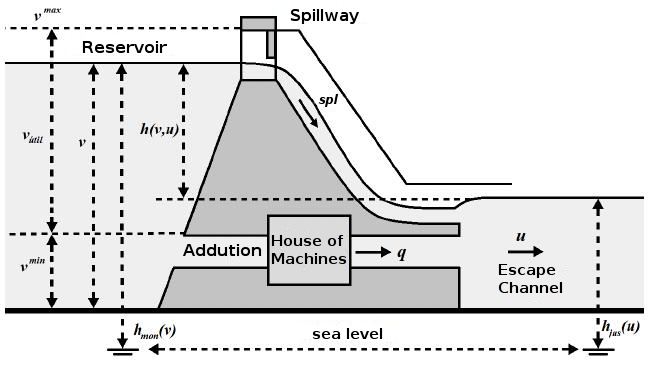
\includegraphics[width=2.5in]{./fig/Componentes-usinas-hidreletricas_en.jpg}
  \label{fig:componentesUsinasHidreletricas}
\end{figure}

\begin{description}[\IEEEsetlabelwidth{$h_{down}(u)$}]
 \item[$v$] volume of the reservoir [$hm^{3}$]
 \item[$v^{max}$] maximum operational volume of the reservoir [$hm^{3}$]
 \item[$v^{min}$] minimum operational volume of the reservoir [$hm^{3}$]
 \item[$v_{u}$] useful volume of the reservoir ($v^{max} - v^{min}$) [$hm^{3}$]
 \item[$q$] flow turbinated by the house of machines (swallowing) [$m^{3}/s$]
 \item[$spl$] flow unloaded through the spillway (spilling) [$m^{3}/s$]
 \item[$u$] flow unloaded by the plant (defluence) ($q + spl$) [$m^{3}/s$]
 \item[$h_{up}(v)$] upstream quote of the reservoir (function of volume) [$m$]
 \item[$h_{down}(u)$] downstream quote of the reservoir (function of defluence) [$m$]
 \item[$h(v, u)$] height of net fall ($h_{up}(v) - h_{down}(u)$) [$m$]
\end{description}

%Vale notar que a vari�vel $q$, a qual representa a vaz�o turbinada, � limitada pelo engolimento m�ximo da usina $q^{max}$, que � a vaz�o turbinada capaz de produzir a pot�ncia m�xima da usina para uma data altura de queda.

It's worth noting that the variable $q$, which represents the turbinated flow, is limited by the maximum swallowing of the plant $q^{max}$, that is the turbinated flow capable of producing the maximum potency of the plant for a given fall height.

%Em um mesmo rio, � comum a constru��o de uma cascata de usinas hidrel�tricas. Dessa forma, a vaz�o descarregada da usina anterior, conhecida como montante, ir� para o reservat�rio da usinas posterior, conhecida como jusante. Essa vaz�o poder� passar novamente por regulariza��o no reservat�rio da usina em jusante.

On the same river, it's common to build a cascade of hydroelectric plants. This way, the unloaded flow from the previous plant, known as upstream, will go to the reservoir of the next plant, known as downstream. This flow can be regulated again by the reservoir of the downstream plant.

%\subsection{Formula��o do Problema de Planejamento da Opera��o Energ�tica}
\subsection{Formulation of the Problem of Energy Operation Planning}

%O planejamento da opera��o energ�tica tem como objetivo minimizar o custo de gera��o de um sistema termel�trico, ao mesmo tempo que mant�m os reservat�rios das usinas hidrel�tricas em alta. Ou seja, temos aqui dois objetivos distintos: minimizar o custo, o qual tem sua por��o vari�vel na gera��o t�rmica complementar, e maximizar o volume final dos reservat�rios. Para resolver esse problema, consideram-se conhecidas as vaz�es afluentes e a demanda e leva-se em conta as caracter�sticas individuais de cada usina hidrel�trica. As fun��es objetivos a serem otimizadas s�o descritas pelo vetor objetivo $\vec{F}$ mostrado na Equa��o \ref{eq:funcoesObjetivo}, onde $CT$ representa a soma dos custos de gera��o de energia por usinas t�rmicas durante todo o per�odo de planejamento (Equa��o \ref{eq:funcaoObjetivoCustoTermico}) e $VF$ � associada ao n�vel dos reservat�rios das hidrel�tricas no �ltimo per�odo de planejamento.

The energy operation planning has the goal of minimizing the generation cost of a hydrothermal system, at the same time that keep the level of reservoirs high. It means that we have two distinct objectives: minimize the cost, which has its variable part in the complementary thermal generation, and maximize the final volume of storage. To solve this problem, we consider the affluences and the demand as known and take into consideration the individual characteristics of each hydroelectric plant. The objective functions to be otimized are described by the objective vector $\vec{F}$ shown in the Equation \ref{eq:funcoesObjetivo}, where $CT$ represents the sum of thermal generation costs during the whole period of planning (Equation \ref{eq:funcaoObjetivoCustoTermico}) and $VF$ is associated with the level of storage of the hydroelectric plants in the last period of planning.

\begin{equation}\label{eq:funcoesObjetivo}
 \vec{F} = \{CT, VF\}
\end{equation}

%O parque termel�trico � considerado como se toda a gera��o el�trica se concentrasse em uma �nica usina, isso se d� pela impossibilidade de se poder atribuir um custo preciso � opera��o da gera��o t�rmica sem considerar diversos outros fatores. Portanto, utiliza-se uma fun��o polinomial para representar o custo da gera��o da energia el�trica, como exibido na Equa��o \ref{eq:custoTermico}.

As the source of thermal energy, we consider as if it is all provided by a single thermal plant. That's because it's impossible to assign the accurate cost of operation of the thermal generation without considering a lot of factors. Therefore, we'll use a polynomial function to represent its generation cost, as shown in the Equation \ref{eq:custoTermico}.

\begin{equation}\label{eq:funcaoObjetivoCustoTermico}
 CT = min \sum_{t=1}^{T} f(gt_{t})
\end{equation}

\begin{equation}\label{eq:custoTermico}
 f(gt_{t}) = \alpha + \beta.gt_{t} + \gamma.gt_{t}^{2} 
\end{equation}

%As fun��es objetivos est�o sujeitas �s seguintes restri��es:
The objective functions are subjected to the following restrictions:

\begin{equation}\label{eq:balanceamentoDeCarga}
 gt_{t} + \sum_{i=1}^{N} gh_{it} - D_{t} - L_{t} = 0
\end{equation}

\begin{equation}\label{eq:limitesGeracaoTermica}
 gt^{min} \leq gt_{t} \leq gt^{max}
\end{equation}

\begin{equation}\label{eq:limitesGeracaoHidreletrica}
 gh_{i}^{min} \leq gh_{it} \leq gh_{i}^{max}
\end{equation}

\begin{equation}\label{eq:geracaoHidraulica}
 gh_{it} = k_{i}.[h_{up}(v_{it}) - h_{down}(q_{it} + spl_{i}) - pc].q_{it}
\end{equation}

\begin{equation}\label{eq:balanceamentoDinamicoDaAgua}
 v_{it} = v_{i,t-1} + y_{it} - q_{it} - spl_{it} + \sum_{m=1}^{\Phi_{i}} (q_{m,t} + spl_{m,t}), m \in \Phi_{i}
\end{equation}

\begin{equation}\label{eq:limitesArmazenamento}
 v_{i}^{min} \leq v_{it} \leq v_{i}^{max}
\end{equation}

\begin{equation}\label{eq:volumeInicial}
 v_{i0} = v_{i}^{ini}
\end{equation}

\begin{equation}\label{eq:volumeFinal}
 v_{iT} = v_{i}^{final}
\end{equation}

\begin{equation}\label{eq:limitesTurbinagem}
 q_{i}^{min} \leq q_{it} \leq q_{i}^{max}(h_{i}(t))
\end{equation}

onde: 

\begin{description}[\IEEEsetlabelwidth{$h_{down}(q_{it} + spl_{it})$}]
 \item[$F$] total thermal cost during the horizon [\$]
 \item[$T$] number of stages of the planning horizon (time interval) [months]
 \item[$t$] index of the time interval [month]
 \item[$N$] number of plants of the system
 \item[$i$] index of the plant of the system
 \item[$gt_{t}$] thermal generation during the interval $t$ [$\overline{\rm MW}$\footnote{One $\overline{\rm MW}$ is the energy equivalent of a source of one $MW$ of potency in a given interval. In this case, we considered one month.}]
 \item[$f(gt_{t})$] cost function of thermal generation in the interval $t$ [\$]
 \item[$gh_{it}$] generation of the plant $i$ during the interval $t$ [$\overline{\rm MW}$]
 \item[$v_{it}$] storage volume of the plant $i$ in the end of interval $t$ [$hm^{3}$]
 \item[$q_{it}$] turbinated flow by the plant $i$ during the interval $t$ [$m^{3}$]
 \item[$spl_{it}$] spilled flow by the plant $i$ during the interval $t$ [$m^{3}$]
 \item[$k_{it}$] producibility of plant $i$
 \item[$h_{up}(v_{it})$] function of the height of upstream of the plant $i$ at the end of the interval $t$ [$m$]
 \item[$h_{down}(q_{it} + spl_{it})$] function of the height of downstream of the plant $i$ at the end of the interval $t$ [$m$]
 \item[$pc$] hydraulic losses
 \item[$y_{it}$] incremental affluent flow of the plant $i$ during the interval $t$ [$m^{3}/s$]
 \item[$\Phi_{i}$] set of plants immediately downstream the plant $i$
 \item[$D_{t}$] demand to be attended during the interval $t$ [$\overline{\rm MW}$]
 \item[$L_{t}$] transmission losses of energy during the interval $t$ [$\overline{\rm MW}$]
 \item[$\alpha, \beta, \gamma$] coefficients of the thermal generation cost function
 \item[$v_{i}^{min},v_{i}^{max}$] minimum and maximum volume of the reservoir of the plant $i$ [$hm^{3}$]
 \item[$v_{i}^{ini},v_{i}^{final}$] initial and final volume of the reservoir of the plant $i$ [$hm^{3}$]
 \item[$q_{i}^{min},q_{i}^{max}$] minimum and maximum turbination of the plant $i$ [$m^{3}$]
 \item[$gh_{i}^{min},gh_{i}^{max}$] minimum and maximum capacity of hydraulic generation of the plant $i$ [$\overline{\rm MW}$]
 \item[$gt_{i}^{min},gt_{i}^{max}$] minimum and maximum capacity of thermal generation [$\overline{\rm MW}$]
 \item[$h_{i}(t)$] fall height of the plant $i$ at the end of the interval $t$ [$m$]
\end{description}

%\section{Descri��o dos Algoritmos Avaliados}
\section{Description of the Evaluated Algorithms}
\label{cap:sistemasHidrotermicos} 

%Foram implementados alguns dos mais eficientes algoritmos de otimiza��o multiobjetivo encontrados na literatura atual na solu��o do Problema do Planejamento Energ�tico de Sistemas Hidrot�rmicos. Tr�s deles s�o baseados em algoritmos evolucion�rios: NSGA-II \cite{deb2002}, SPEA2 \cite{zitzler2001} e MOCell \cite{nebro2006} \cite{nebro2007}; e dois s�o baseados em enxame de part�culas: OMOPSO \cite{reyes2005} e SMPSO \cite{nebro2009}.

Some of the most efficient algorithms of multi objective optimization found in the literature currently were implemented to solve the Problem of Energy Operation Planning of Hydrothermal Systems. Three of them are based on evolutionary algorithms: NSGA-II \cite{deb2002}, SPEA2 \cite{zitzler2001} e MOCell \cite{nebro2006} \cite{nebro2007}; and two of them are based on particle swarm optimization: OMOPSO \cite{reyes2005} e SMPSO \cite{nebro2009}.

%NSGA-II � um algoritmo gen�tico baseado na obten��o de uma nova popula��o da popula��o original atrav�s da aplica��o dos operadores gen�ticos (sele��o, cruzamento e muta��o). Entretanto, ao inv�s de passar essa nova popula��o diretamente para a pr�xima itera��o, ela � combinada com a anterior e as solu��es s�o ordenadas por um rank. Assim, apenas as melhores solu��es dessa combina��o s�o escolhidas para gerar uma nova popula��o. Caso aconte�a algum empate na avalia��o do rank, uma estimativa de densidade baseada em crowding distance dos individuos ao redor � usada para selecionar as solu��es mais promissoras.

NSGA-II is an genetic algorithm based in obtaining the new population from the original one through the application of the genetic operators (selection, crossover and mutation). However, instead of passing the new population directly to the next iteration, it's combined with the previous one and the solutions are sorted by a rank. This way, only the best solutions of this combination are chosen to generate a new population. IIn case of a tie happen in the evaluation of the rank, the density estimation based on crowding distance of the surrounding individuals is used to select the most promising solutions.

%SPEA2 tamb�m � um algoritmo gen�tico. Por�m, nesse algoritmo, cada indiv�duo tem um valor de fitness calculado pela soma de seu fitness puro com uma estima��o de densidade. O algoritmo aplica os operadoradores gen�ticos para preencher um arquivo de indiv�duos. Ent�o, os indiv�duos n�o dominados da combina��o da popula��o original com o arquivo s�o copiados para uma nova popula��o. Se o n�mero de indiv�duos n�o dominados for maior do que o tamanho da popula��o, um operadora de truncamento baseado no c�lculo de KNN (K-th Nearest Neighbor) � usado. Dessa forma, os ind�viduos com menores dist�ncias qualquer outro indiv�duo s�o selecionados.

SPEA2 is also a genetic algorithm. However, in this algorithm, each individual has a fitness value calculated by the sum of its raw fitness with a the density estimation. The algorithm applies the genetic operators to fulfill the archive of individuals. Then, the non dominated individuals of the combination of the original population with the archive are copied to the new population. If the number of non dominated individuals is greater than the size of the population, a truncation operator based on the KNN (K-th Nearest Neighbor) is used. This way, the individuals with the lowest distances to any other individual are selected.

%MOCell � um algoritmo gen�tico celular (cGA). Ele inclui um arquivo externo para guardar solu��es n�o dominadas encontradas durante sua execu��o. Esse arquivo faz uso de crowding distance do NSGA-II para manter a diversidade.

MOCell is a cellular genetic algorithm (cGA). It includes an external archive to keep the non dominated solutions found during the execution. This archive uses the crowding distance of NSGA-II to preserve the diversity.

%OMOPSO � um algoritmo multiobjetivo de enxame de part�culas. Assim como o MOCell, ele faz uso de um arquivo externo para guardar solu��es n�o dominadas encontradas durante sua execu��o, tamb�m com crowding distance do NSGA-II para filtrar as melhores solu��es. Al�m disso, diferente de outros algoritmos de enxame de part�culas, ele faz uso de muta��o para acelerar a converg�ncia do enxame. Seu arquivo externo faz uso do conceito de domin�ncia $\epsilon$ para limitar o n�mero de solu��es guardadas.

OMOPSO is a multi objective particle swarm optimization algorithm. Like MOCell, it uses an external archive to keep the non dominated solutions found during the execution and the crowding distance of NSGA-II to filter the best solutions. Besides that, different from other algorithms of particle swarm optimization, it uses mutation to accelerate the convergence of the swarm. Its external archive uses the concept of $\epsilon$ dominance to limit the number of solutions kept.

%SMPSO � um variante do OMOPSO com a ado��o de uma nova abordagem de constri��o de velocidade com o fim de limitar a velocidade das part�culas. Esse constri��o evita que a velocidade das part�culasalcance valores altos demais e pequenos demais, o que pode prejudicar a busca. Fora isso, a outra diferen�a est� no operador de muta��o utilizado pelo OMOPSO e o SMPSO, como ser� visto na Tabela \ref{table:parametrosUtilizados}.

SMPSO is a variant of the OMOPSO with the adoption of a new approach to constrict the speed of the particles. This constriction avoids that their speed reaches values too high and too low, which could harm the search. Beyond that, the other difference is in the mutation operator used by OMOPSO and SMPSO, as will be shown in the Table \ref{table:parametrosUtilizados}.
%\section{Estudos de Caso}
\section{Study Cases}
\label{cap:estudosDeCaso}

%\subsection{Cen�rio de Teste}
\subsection{Test Scenario}

%O problema do planejamento energ�tico foi simulado para um conjunto de 8 usinas hidrel�tricas reais do sistema brasileiro, utilizando dados reais de tr�s per�odos de 60 meses: maio/1951 a abril/1956, maio/1961 a abril/1966 e maio/1980 a abril/1985. As usinas est�o localizadas na Bacia do Rio Grande e Parana�ba. Elas est�o esquematizadas na Figura \ref{fig:conjuntoUsinas} e suas caracter�sticas s�o apresentadas na Tabela \ref{table:conjuntoUsinas}. Os tr�s per�odos utilizadados aqui, tamb�m foram utilizados em \cite{gomides2012} e \cite{silva2014} devido �s suas caracter�sticas �nicas e relevantes para a otimiza��o. O primeiro per�odo � determinado por meses de seca, a vaz�o dos rios estava baixa e o custo de gera��o el�trica consequentemente se tornou maior, esse � o per�odo mais importante utilizado neste estudo de caso, uma vez que � o que mais apresenta restri��es � otimiza��o do problema. O segundo e o terceiro per�odo s�o caracterizados por vaz�es m�dias e altas dos rios, respectivamente.

The problem of energy planning was simalted for a group of 8 real hydroelectric plants of the brazilian system, using real data of three periods of 60 months: from May/1951 to April/1956, from May/1961 to April/1966 and from May/1980 to April/1985. The plants are located in the Basin of the Rio Grande and Parana�ba. Their topology are shown in the Figure \ref{fig:conjuntoUsinas} and their characteristics are presented in the Table \ref{table:conjuntoUsinas}. These plants and periods were also used in \cite{gomides2012} and \cite{silva2014} because of their unique and relevant characteristics for the otimization. The first period is determined by dry months, when the rivers' flow were low and the cost of generation was consequently higher. This was the most important period of the study case, since it presents more restrictions to optimize the problem. The second and the third periods presents medium and high rivers' flow, respectively.

\begin{figure}[!t]
  \centering
  \caption{Topology used in the study case}
  \includegraphics[width=2.5in]{./fig/Conjunto-Usinas_en.pdf}
  \label{fig:conjuntoUsinas}
\end{figure}

\begin{table}[!t]
\caption{Group of hydroelectric plants of the study case}
\label{table:conjuntoUsinas}
\centering
\begin{tabular}{lcc}
    \hline
    Plant                 & Potency (MW)   & Reservoir (hm$^{3}$)     \\ \hline
    Furnas                & $1,312$        & $22,950$                 \\
    Mascarenhas de Moraes & $478$          & $4,040$                  \\
    Marimbondo            & $1,488$        & $6,150$                  \\
    �gua Vermelha         & $1,396.2$      & $11,025$                 \\
    Emborca��o            & $1,192$        & $17,725$                 \\
    Itumbiara             & $2,280$        & $17,027$                 \\
    S�o Sim�o             & $1,710$        & $12,540$                 \\
    Ilha Solteira         & $3,444$        & $21,046.359375$          \\ \hline
    Total                 & $13,300.2$     & $112,503.359375$         \\ \hline
\end{tabular}
\end{table}

%Os estudos de casos precisam simular o atendimento da demanda por energia el�trica mensal, essa demanda de mercado ($D_{t}$) deve ser atendida pela combina��o das gera��es hidr�ulicas e t�rmicas. Para simplificar o processo de simula��o, a demanda foi considerada constante e com valor $D_{t} = 14,000$. O mesmo valor foi utilizado nos estudos de \cite{gomides2012} e \cite{silva2014}. Em rela��o �s chuvas e vaz�es, optou-se pela utiliza��o de dados reais dos per�odos citados. Assim, � poss�vel calcular a gera��o hidrel�trica, obter a gera��o t�rmica necess�ria para se complementar a demanda e por fim calcular o custo t�rmico.

The study cases must simulate the attending of the monthly demand of electric energy. This demand ($D_{t}$) must be attended by the hydroelectric and thermal generations. To simplify the simulation process, the demand was considered constant and with de value $D_{t} = 14,000$. The same value was used in the studies of \cite{gomides2012} and \cite{silva2014}. Regarding the rains and flows, we opted to use real data from the cited periods. This way, it's possible to calculate the hydroelectric generation, obtain the thermal generation necessary to attend the demand and lastly calculate the thermal cost.

%Para o c�lculo do custo t�rmico ($CT$), utilizou-se a Equa��o \ref{eq:calculoCustoTermico}, onde $gt_{t}$ representa a gera��o t�rmica total. Essa equa��o � uma adapta��o da Equa��o \ref{eq:custoTermico}, onde $\alpha = \beta = 0$ e $\gamma = \frac{1}{2}$.

To calculate the thermal cost ($CT$), we used the Equation \ref{eq:calculoCustoTermico}, where $gt_{t}$ represents the total thermal generation. This equation is an adaptation of the Equation \ref{eq:custoTermico}, where $\alpha = \beta = 0$ and $\gamma = \frac{1}{2}$.

\begin{equation}\label{eq:calculoCustoTermico}
 CT = f(gt_{t}) = \frac{1}{2}(gt_{t})^{2}
\end{equation} 

%\subsection{Arquitetura do Sistema}
\subsection{System Architecture}

%Para implementa��o dos algoritmos, foi utilizada a linguagem Java em conjunto com o framework JMetal \cite{durillo2011}, o qual disponibiliza diversos algoritmos de otimiza��o orientados a objetos e toda um l�gica de execu��o dos estudos com a cria��o de um relat�rio dos resultados ao fim. Seguindo a API desse framework, cada part�cula do enxame/elemento da popula��o foi implementada como um $DoubleSolution$, o qual � um objeto contendo um vetor de n�meros reais. Para o problema apresentado, cada poss�vel solu��o foi composta por um vetor de 480 n�meros reais, os quais possuiam valores entre 0 e 1. Esses valores representam a turbinagem normalizada de determinada usina do conjunto em determinado m�s dentro do per�odo. Como cada per�odo possui 60 meses e existem 8 usinas nesse estudo de caso, o vetor foi organizado em grupos de 60 n�mero reais. Vale notar que a normaliza��o dessa turbinagem ocorre atrav�s da divis�o da quantidade turbinada pelo engolimento m�ximo da usina correspondente.

To implement the algorithms, we used the Java language with the framework JMetal \cite{durillo2011}, which provides a lot of object oriented optimization algorithms and a toolkit to manage the study cases and generate reports. Following this framework's API, each particle of the swarm/element of the population was implemented as an $DoubleSolution$, which is an object containing an array of real numbers. Each possible solution was composed of an array of 480 real numbers, each of them having values between 0 and 1. These values represent the normalized turbination of each plant of the group in each month of the period. Since each period has 60 months and there are 8 plants, the array was organized in 8 groups of 60 real numbers. It's woth noting that the normalization of the turbination is done through the division of the turbination by the maximum swallowing of the corresponding plant.

%Com essa composi��o das poss�veis solu��es, torna-se poss�vel os c�lculos que levam �s duas vari�veis a serem otimizadas: custo de opera��o e armazenamento final dos reservat�rios. Esses c�lculos foram executados para cada part�cula do enxame/elemento da popula��o pelo simulador de opera��o de usinas hidrel�tricas disponibilizado por \cite{ramos2017}. Esse simulador possui um banco de dados com os dados das usinas hidrel�tricas estudadas, bem como os dados de aflu�ncias ocorridas nos per�odos do estudo. Assim, atrav�s da turbinagem de cada usina em cada m�s em conjunto com os dados de aflu�ncias, ele � capaz de calcular os resultados para aquele m�s. O simulador automaticamente reutiliza esses resultados para o c�lculo dos meses seguintes e tamb�m das usinas a jusante. Assim, ele retorna os resultados de todos os meses de todas as usinas para dada simula��o. Por fim, utiliza-se a pot�ncia total gerada e a demanda para o c�lculo do custo de gera��o t�rmica (a ser minimizada) e soma-se o armazenamento final de todas as usinas (a ser maximizado).

With this composition of the possible solutions, it's possible to calculate the two objective variables: operational cost and final volume of the reservoirs. This calculation was executed for each particle of the swarm/element of the population by the simulator of hydroelectric plant's operation from \cite{ramos2017}. This simulator has a database of the data of the studied hydroelectric plants and the affluences data of the studied periods. This way, with the turbination of each plant at each month and the affluences data, it's capable of calculating the results of each month for each plant. The simulator automatically uses these results to calculate the results of the next months and considers their effects to the downstream plants. Lastly, we use the total generated potency and the demand to calculate the thermal generation cost (to be minimized) and we sum up the final volume of the reservoirs of all the plants (to be maximized).

%\subsection{Par�metros Utilizados nos Algoritmos}
\subsection{Parametrization of the Algorithms}
\label{sec:parametrosUtilizados}

%Com o fim de tornar a compara��o entre esses algoritmos mais justa, foram utilizados os par�metros exibidos na Tabela \ref{table:parametrosUtilizados}. Esses foram os mesmos utilizados na avalia��o desses mesmos algoritmos (com a adi��o do AbYSS) feita por \cite{nebro2009} atrav�s de conhecidos benchmarks.

With the goal of making the comparison of the algorithms fair, we used the parametrization shown in the Table \ref{table:parametrosUtilizados}. This parametrization was the same used in the evaluation of these algorithms (plus the AbYSS) done by \cite{nebro2009} through known benchmarks.

\begin{table}[!t]
\caption{Parametrization of the Algorithms ($L$ = individual length)}
\label{table:parametrosUtilizados}
\centering
\begin{tabular}{ll}
    \hline
    \multicolumn{2}{l}{Parametrization used in NSGA-II}                      \\ \hline
    Population Size                & 100 individuals                         \\
    Selection of Parents           & binary tournament + binary tournament   \\
    Recombination                  & simulated binary (SBX), $p_{c} = 0.9$   \\
    Mutation                       & polynomial, $p_{m} = 1.0/L$             \\
    \hline
    \multicolumn{2}{l}{Parametrization used in SPEA2}                        \\ \hline
    Population Size                & 100 individuals                         \\
    Selection of Parents           & binary tournament + binary tournament   \\
    Recombination                  & simulated binary (SBX), $p_{c} = 0.9$   \\
    Mutation                       & polynomial, $p_{m} = 1.0/L$             \\
    \hline
    \multicolumn{2}{l}{Parametrization used in MOCell}                       \\ \hline
    Population Size                & 100 individuals(10 x 10)                \\
    Neighborhood                   & 1-hop neighbours (8 surrounding solutions)\\
    Selection of Parents           & binary tournament + binary tournament   \\
    Recombination                  & simulated binary (SBX), $p_{c} = 0.9$   \\
    Mutation                       & polynomial, $p_{m} = 1.0/L$             \\
    Archive size                   & 100 individuals                         \\
    \hline
    \multicolumn{2}{l}{Parametrization used in OMOPSO}                       \\ \hline
    Swarm Size                     & 100 particles                           \\
    Mutation                       & uniform + non-uniform                   \\
    Leaders Size                   & 100                                     \\
    \hline
    \multicolumn{2}{l}{Parametrization used in SMPSO}                        \\ \hline
    Swarm Size                     & 100 particles                           \\
    Mutation                       & polynomial, $p_{m} = 1.0/L$             \\
    Archive size                   & 100 individuals                         \\
    \hline
\end{tabular}
\end{table}

%Al�m desses par�metros, existe um par�metro impl�cito utilizado na muta��o polinomial e na recombina��o bin�ria simulada (SBX), operadores presentes em todos os algoritmos, com exce��o do OMOPSO que n�o possui esses operadores e o SMPSO que possui apenas a muta��o polinomial. Esse par�metro � chamado de �ndice de distribui��o, possui valor real acima de $0$ e geralmente assume o valor padr�o de $20.0$. Esse �ndice trabalha nesses operadores de muta��o e recombina��o de tal forma que, quanto menor seu valor, maior ser� a diversidade dos novos indiv�duos criados, aumentando a explora��o do ambiente por parte dos algoritmos de busca. Para este trabalho, tr�s valores diferentes foram adotados na avalia��o dos algoritmos: $1.0$, $10.0$ e $20.0$. Dessa forma, cada algoritmo (que possua esse par�metro) foi avaliado tr�s vezes distintas, cada uma com um desses valores de �ndice de distribui��o.

Beyond these parameters, there's an implicit parameter used by the polynomial mutation and the simulated binary recombination (SBX), operators used by most of these algorithms. This parameter is known as distribution index and it assumes a real number above $0.0$ as its value, usually having the default value of $20.0$. The distribution index works in those mutation and recombination operators in a way that the lesser its value, the greater will be the diversity of the new individuals created, which increases the exploration of the enviroment by the search algorithms. For this article, three different values were adopted in the evaluation of the algorithms: $1.0$, $10.0$ and $20.0$. This way, each algorithm (which contains this parameter) was evaluated three times, one for each value of distribution index.

%Por fim, os algoritmos testados continham uma popula��o de 100 part�culas/indiv�duos, como mostrado na Tabela \ref{table:parametrosUtilizados}, e cada execu��o continha 500 itera��es. Foram realizadas 25 execu��es de cada par de algoritmo e �ndice de distribui��o para cada periodo considerado neste trabalho.

Lastly, the evaluated algorithms presents a population of 100 particles/individuals, as shown in the Table \ref{table:parametrosUtilizados}, and each execution has 500 iterations. Each pair of algorithm and distribution index was executed 25 times for each period.
%\section{Resultados e Discuss�es}
\section{Results and Discussion}
\label{cap:resultadosDiscussoes}

%Deseja-se avaliar os resultados obtidos por esses algoritmos de acordo com os dois objetivos utilizados: diminuir os custos de gera��o t�rmica e aumentar o volume final dos reservat�rios das usinas. Para facilitar a visualiza��o das frentes de pareto, o volume final foi convertido em porcentagem, indo de 0 a 100\%. Al�m disso, os valores do volume final receberam valores negativos, sendo apresentados de -100 at� 0\%.

We want to evaluate the results of the algorithms according to the goals: to decrease the thermal generation costs and to increate the final volume of the reservoirs of the plants. To make it easier to visualize the pareto front in the figures, the final volume is given in percentage. Beyond that, it's presented in negative numbers, from -100\% to 0\%.

%Os valores obtidos pelos algoritmos utilizados ser�o comparados entre si atrav�s de conhecidas m�tricas de qualidade, al�m da apresenta��o dos gr�ficos de suas frentes de pareto junto � frente de refer�ncia. Deve-se notar que, por n�o possuirmos uma frente de pareto de refer�ncia ideal com o melhor resultado poss�vel, foi criada uma a partir dos melhores resultados de todas execu��es de todos os algoritmos.

These results will be compared through known quality indicators and graphics showing the obtained pareto fronts with the reference pareto front. It's worth noting that, since we don't have the real pareto front with the optimum solutions, a reference pareto front was created with the best results of all the executions of all the algorithms. 

%\subsection{Per��odo 1951-1956}
\subsection{1951-1956}

%Tratando-se de um per�odo de seca, espera-se maior dificuldade na otimiza��o da opera��o das usinas nesse per�odo. Portanto, � um per�odo chave na compara��o entre os algoritmos.

Being a dry period, we expect it to be harder for the plants' operation to be optimized. So, this is a key period in the comparison of the algorithms.

%A Tabela \ref{table:epPeriodo1} apresenta a mediana e o desvio do valor \textit{I}$^{1}_{\epsilon+}$ obtido em todas execu��es de cada algoritmo para esse per�odo. Esse indicador mostra o qu�o pr�xima a frente de pareto obtida est� da frente de pareto de refer�ncia, sendo melhor o resultado quanto menor o valor. Nessa tabela tamb�m est� indicado em cinza escuro e cinza claro o melhor e o segundo melhor resultado, respectivamente. Uma �ltima observa��o importante � que os valores apresentados entre par�nteses ap�s o nome de cada algoritmo referem-se ao valor do �ndice de distribui��o utilizado nas opera��es de cruzamento e muta��o, como discutido na Se��o \ref{sec:parametrosUtilizados}. As tabelas seguintes ser�o apresentadas de maneira semelhante.

The Table \ref{table:epPeriodo1} presents the mean and the standard deviation of the \textit{I}$^{1}_{\epsilon+}$ Indicator obtained in all the executions of each algorithm of this period. This indicator shows how close the pareto front is in relation to the reference pareto front, being that the smaller the value the best is the result. In this table, the best and the second best results are highlighted with dark and light gray, respectively. It's also important to note that the values presented between parenthesis after the name of each algorithm refers to the value of the distribution index used in the combination and mutation operators, as discussed in the Section \ref{sec:parametrosUtilizados}. The other tables follow the same pattern.

\begin{table}[!t]
\caption{Mean and Standard Deviation of Additive Epsilon Indicator (\textit{I}$^{1}_{\epsilon+}$) of the first period}
\label{table:epPeriodo1}
\centering
\begin{tabular}{ll}
    ~                             & Mean and Standard Deviation               \\ \hline
    OMOPSO                        & $  2.52e-01_{ 4.5e-02}$                   \\
    SMPSO (1.0)                   & $  3.31e-01_{ 4.6e-02}$                   \\
    SMPSO (10.0)                  & $  3.29e-01_{ 4.9e-02}$                   \\
    SMPSO (20.0)                  & $  3.43e-01_{ 4.4e-02}$                   \\
    NSGA-II (1.0)                 & \cellcolor{gray25}$  1.40e-01_{ 2.3e-02}$ \\
    NSGA-II (10.0)                & $  2.20e-01_{ 4.7e-02}$                   \\
    NSGA-II (20.0)                & $  2.15e-01_{ 4.7e-02}$                   \\
    SPEA2 (1.0)                   & $  1.72e-01_{ 3.1e-02}$                   \\
    SPEA2 (10.0)                  & $  2.10e-01_{ 3.0e-02}$                   \\
    SPEA2 (20.0)                  & $  2.08e-01_{ 3.1e-02}$                   \\
    MOCell (1.0)                  & \cellcolor{gray95}$  1.07e-01_{ 2.7e-02}$ \\
    MOCell (10.0)                 & $  2.24e-01_{ 5.0e-02}$                   \\
    MOCell (20.0)                 & $  2.60e-01_{ 4.3e-02}$                   \\
\end{tabular}
\end{table}

%A primeira an�lise que pode-se fazer ao observarmos a Tabela \ref{table:epPeriodo1} � que, de modo geral, valores menores para o �ndice de distribui��o geraram melhores resultados. Essa afirma��o � verdadeira para todos algoritmos, por�m, tendo uma ressalva em rela��o ao algoritmo SMPSO, que obteve resultados muito pr�ximos com os �ndices de valor $1.0$ e $10.0$. Nota-se que apesar de uma mediana com valor ligeiramente menor para o �ndice $10.0$, seu desvio padr�o tamb�m � ligeiramente maior. Assim, indica-se baixa varia��o nos resultados do algoritmo SMPSO com rela��o � altera��o do par�metro de �ndice de distribui��o de seu operador de muta��o.

The first analysis to be done after observing the Table \ref{table:epPeriodo1} is that, in general, smaller values of the distribution index generated better results. This affirmation is true for all the algorithms, even though the results of the SMPSO were very close for the values of $1.0$ and $10.0$ of distribution index. So, we can state that, in this case, the SMPSO suffers little influence of the variation of the distribution index of its mutation operator.

%Por outro lado, a diferen�a nos resultados dos outros algoritmos � consider�vel. Observa-se grande diferen�a entre os resultados dos algoritmos com �ndice $1.0$ em rela��o aos outros valores e uma pequena diferen�a entre os valores $10.0$ e $20.0$. Por fim, conclui-se que, pelo menos em rela��o a esse per�odo e esse indicador, o valor $1.0$ � o melhor valor encontrado para a opera��o desses algoritmos com esse problema espec�fico. Lembrando que o valor desse par�metro funciona de tal forma que quanto menor ele seja, mais distantes poder�o ser as solu��es criadas atrav�s de cruzamentos e muta��es. Isso permite maior explora��o em troca de uma converg�ncia mais lenta.

On the other hand, the difference of the results of the other algorithms are substantial. It's noticiable the great difference between the results of the algorithms with distribution index of $1.0$ and the other values. The difference between $10.0$ and $20.0$ is smaller. Lastly, we can deduce that, at least for this period and this indicator, the value $1.0$ is the best one found for the operation of these algorithms with this problem.

%Al�m disso, podemos notar que o claro vencedor nesse per�odo de acordo com esse indicador foi o algoritmo MOCell, seguido pelo NSGA-II. Vale lembra que o \textit{I}$^{1}_{\epsilon+}$ mede apenas a converg�ncia desses algoritmos em rela��o a frente de pareto de refer�ncia. Ou seja, mede o qu�o pr�ximo seus resultados ficaram dessa refer�ncia, sendo melhor um resultado menor.

%Com o SPEA2 como terceiro colocado, podemos notar que a fam�lia de algoritmos evolucion�rios parece ter se adaptado melhor a esse problema do que aqueles de enxame de enxames, visto que seus todos seus representantes obtiveram resultados melhores do que o OMOPSO e o SMPSO.

Beyond that, we can notice that the clear winner of this period according to the \textit{I}$^{1}_{\epsilon+}$ Indicator was the MOCell, followed by NSGA-II. Having the SPEA2 as the third best, we can claim that the evolutionary algorithms had a better adaptation for this problem than the particle swarm optimization algorithms, since all the evolutionary algorithms had better results than both OMOPSO and SMPSO.

%Voltando nossa aten��o aos algoritmos de enxame de part�culas, o OMOPSO obteve melhor converg�ncia que seu sucessor, SMPSO. Talvez, isso se deva �s restri��es de velocidade impostos �s part�culas pelo SMPSO. Afinal, como pudemos notar, uma maior explora��o do espa�o de busca rendeu melhores resultados aos demais algoritmos.

Turning attention to the particle swarm optimization algorithms, OMOPSO obtained a better convergence that its successor: SMPSO. Maybe, it's because of the speed constriction of the particles of SMPSO. After all, we can notice that a greater exploration of the environment yielded good results to the other algorithms, as pointed by the variation of the distribution index.

%Apesar desses resultados, a converg�ncia n�o � o �nico aspecto importante em uma frente de pareto. Devemos observar a diversidade das solu��es apresentadas. Afinal, o grande prop�sito na solu��o de problemas multiobjetivos � gerar diversas op��es aos operadores do sistema, para que esses possam decidir a solu��o a ser adotada. Para avaliar esse aspecto das solu��es, disponibiliza-se a Tabela \ref{table:spreadPeriodo1}.

Despite these results, the convergence isn't the only important aspect of a pareto front. We should also observe the diversity of the obtained solutions. In the end, the great purpose of the multi objective optimization is to generate various options for the system's operators, so they can decide the solution to be adopted. To evaluate this aspect of the solutions, there's the Table \ref{table:spreadPeriodo1}.

\begin{table}[!t]
\caption{Mean and Standard Deviation of the SPREAD Indicator ($\Delta$) of the first period}
\label{table:spreadPeriodo1}
\centering
\begin{tabular}{ll}
    ~              & Mean and Standard Deviation               \\ \hline
    OMOPSO         & $  5.99e-01_{ 4.8e-02}$                   \\
    SMPSO (1.0)    & \cellcolor{gray95}$  5.75e-01_{ 7.0e-02}$ \\
    SMPSO (10.0)   & \cellcolor{gray25}$  5.80e-01_{ 9.6e-02}$ \\
    SMPSO (20.0)   & $  5.85e-01_{ 1.1e-01}$                   \\
    NSGA-II (1.0)  & $  6.50e-01_{ 4.3e-02}$                   \\
    NSGA-II (10.0) & $  7.08e-01_{ 7.4e-02}$                   \\
    NSGA-II (20.0) & $  7.18e-01_{ 6.9e-02}$                   \\
    SPEA2 (1.0)    & $  7.38e-01_{ 7.6e-02}$                   \\
    SPEA2 (10.0)   & $  7.62e-01_{ 5.5e-02}$                   \\
    SPEA2 (20.0)   & $  7.48e-01_{ 4.8e-02}$                   \\
    MOCell (1.0)   & $  6.26e-01_{ 1.0e-01}$                   \\
    MOCell (10.0)  & $  6.93e-01_{ 6.9e-02}$                   \\
    MOCell (20.0)  & $  6.64e-01_{ 1.0e-01}$                   \\
\end{tabular}
\end{table}

%Com os resultados do Indicador $\Delta$, notamos resultados opostos aos encontrados com o Indicador \textit{I}$^{1}_{\epsilon+}$. Isso mostra que apesar de pior converg�ncia dos algoritmos de enxame de part�culas, eles obtiveram melhor diversidade de solu��es do que aqueles da fam�lia de algoritmos evolucion�rios. Nesse quesito, destaca-se o SMPSO, que obteve a melhor diversidade com todos os valores do �ndice de distribui��o, ultrapassando seu antecessor, OMPSO. J� dentre os algoritmos evolucion�rios, novamente o MOCell se saiu melhor que os outros. Sendo novamente seguido pelo NSGA-II e por �ltimo o SPEA2.

With the values of $\Delta$ Indicator, it's noticeable that the results were the oposite of what was found with the \textit{I}$^{1}_{\epsilon+}$ Indicator. It shows that despite the worst convergence of the particle swarm algorithms, they obtained a better diversity of solutions than what the evolutionary algorithms achieved. At this matter, the SMPSO is highlighted for achieving a greater diversity with all of the distribution indexes, surpassing its predecessor: OMOPSO. Among the evolutionary algorithms, the MOCell turned out better than the others once again. Also, the NSGA-II was once more better than the SPEA2.

%Quanta � an�lise dos valores de �ndice de distribui��o, em mais um indicador tivemos o mesmo resultado: o valor menor obteve melhores resultados. Isso indica que realmente uma explora��o mais intensa do espa�o de solu��es � algo ben�fico na solu��o desse problema espec�fico.

Regarding the analysis of the distribution index values, the same result was obtained: the smallest value achieved the best results. It reinforces that a more intensive exploration of the search space of solutions is benefitial to solve this problem.

\begin{table}[!t]
\caption{Mean and Standard Deviation of the Hypervolume Indicator (HV) of the first period}
\label{table:hvPeriodo1}
\centering
\begin{tabular}{ll}
    \hline
    ~              & Mean and Standard Deviation               \\ \hline
    OMOPSO         & $  4.80e-01_{ 4.3e-02}$                   \\
    SMPSO (1.0)    & $  4.02e-01_{ 3.1e-02}$                   \\
    SMPSO (10.0)   & $  3.85e-01_{ 4.1e-02}$                   \\
    SMPSO (20.0)   & $  3.96e-01_{ 3.8e-02}$                   \\
    NSGA-II (1.0)  & \cellcolor{gray95}$  6.25e-01_{ 1.8e-02}$ \\
    NSGA-II (10.0) & $  5.91e-01_{ 3.1e-02}$                   \\
    NSGA-II (20.0) & $  5.95e-01_{ 2.7e-02}$                   \\
    SPEA2 (1.0)    & $  5.99e-01_{ 1.9e-02}$                   \\
    SPEA2 (10.0)   & $  6.01e-01_{ 2.5e-02}$                   \\
    SPEA2 (20.0)   & \cellcolor{gray25}$  6.02e-01_{ 2.2e-02}$ \\
    MOCell (1.0)   & $  5.97e-01_{ 2.6e-02}$                   \\
    MOCell (10.0)  & $  5.47e-01_{ 3.3e-02}$                   \\
    MOCell (20.0)  & $  5.04e-01_{ 3.9e-02}$                   \\
\end{tabular}
\end{table}

%Para continuar a an�lise desse per�odo, a Tabela \ref{table:hvPeriodo1} mostra o resultados dos algoritmos para o Indicador de Hipervolume. Esse indicador tem a propriedade �nica que avaliar ao mesmo tempo a converg�ncia, a diversidade a ainda a cardinalidade das solu��es. Esse indicador mede o tamanho do espa�o objetivo coberto pela aproxima��o da frente de pareto em rela��o � frente de pareto de refer�ncia. Isso � feito atrav�s de um ponto de refer�ncia adotado. Note ainda que, diferente dos indicadores anteriores, esse tem como melhor valor aqueles maiores.

To continue the analysis of this period, the Table \ref{table:hvPeriodo1} shows the results of the algorithms for the Hypervolume Indicator. This indicator has an unique property of evaluate at the same time the convergence, the diversity and also the cardinality of the solutions. It measures the size of the objective space covered by the pareto front in relation to the reference pareto front. It's done through a reference point adopted. It's worth noting that different from the previous indicators, the higher the better the value of this indicator.

%Ao observarmos os resultados desse indicador, notamos que novamente os algoritmos evolucion�rios obtiveram melhores resultados que os de enxame de part�culas. Por�m, esse indicador muda um pouco a ordem dos melhores algoritmos. Nesse caso, o NSGA-II obteve o melho resultado de todos, sendo seguido, dessa vez, pelo SPEA2 e por �ltimo o MOCell, que havia obtido os melhores resultados de acordo com as m�tricas anteriores. Por�m, a diferen�a dos resultados desses tr�s algoritmos � pequena de acordo com essa m�trica.

Observing the results of this indicator, it's noticiable that one more time the evolutionary algorithms achieved better results than the particle swarm optimization algorithms. However, the order of the best algorithms has changed. In this case, the NSGA-II obtained the best result, followed by SPEA2 and MOCell, which had the best results according to the previous indicators. Nevertheless, the difference of the results is tiny for this three algorithms according to HV Indicator.

%Voltando nossa aten��o aos algoritmos de enxame de Part�culas, notamos que novamente o OMOPSO superou seu sucessor, SMPSO. Seu resultado foi razoavelmente melhor nessa m�trica, assim como na \textit{I}$^{1}_{\epsilon+}$. Isso indica que, em rela��o a seu antecessor, o SMPSO conseguiu ser melhor apenas na distribui��o das solu��es.

Turning our attention to the particle swarm algorithms, once again the OMOPSO surpassed its successor: SMPSO. Its result was fairly better with this indicator, as it was with \textit{I}$^{1}_{\epsilon+}$. This indicates that, related to its predecessor, the SMPSO was better only in the diversity of the solutions.

%Para essa m�trica, houve grande diferen�a ao analisarmos os valores de �ndice de distribui��o. N�o houve mais o padr�o de que um menor �ndice rendesse melhores resultados. Esse comportamento variou de acordo com o algoritmo estudado. Sendo que enquanto o melhor valor para o NSGA-II foi de $1.0$, o melhor valor do SPEA2 foi justamente o oposto: $20.0$. J� no caso do MOCell, n�o s� o valor de $1.0$ foi melhor, como os outros valores geraram resultados consideravelmente inferiores em rela��o � essa m�trica.

For this metric, there's a great difference in the analysis of the distribution index values. There wasn't the same pattern of the smallest value generating the best results. This behavior varied according to the studied algorithm. While the best value for NSGA-II was $1.0$, the best value for SPEA2 was exactly the oposite: $20.0$. In the case of the MOCell, the $1.0$ not only was the best, but also the other values generated fairly worse results according to this indicator.

%Se compararmos os melhores resultados para cada algoritmo, o NSGA-II saiu vencedor com uma consideravel vantagem. Enquanto isso, SPEA2 e MOCell obtiveram resultados bem pr�ximos. J� o OMOPSO e o SMPSO obtiveram resultados bem inferiores em rela��o aos algoritmos evolucion�rios.

Comparing the best results of each algorithm, the NSGA-II was the winner with a substantial advantage. While SPEA2 and MOCell achieved close results. The worst results were from OMOPSO and SMPSO, that achieved poor results compared to the evolutionary algorithms.

%Com o estudo dessas tr�s m�tricas, podemos concluir que os algoritmos evolucion�rios obt�m melhor converg�ncia da frente de pareto, enquanto os de enxame de part�culas obt�m solu��es mais distribu�das. Por�m, o resultado geral � que os algoritmos evolucion�rios se mostraram mais eficientes.

With the study of these three metrics, we can conclude that the evolutionary algorithms obtained better convergence of the pareto front, while the particle swarm algorithms achieved the best diversity of solutions. However, the general result is that the evolutionary algorithms are more efficient to solve this problem.

%Al�m desses resultados gerais, podemos observar uma inconsist�ncia entre os indicadores. Apesar de ser considerado melhor tanto pelo \textit{I}$^{1}_{\epsilon+}$ quanto pelo $\Delta$, que tratam separadamente converg�ncia e distribui��o, o MOCell caiu para a terceira melhor op��o quando avaliado pelo Hipervolume, que trata ambos aspectos ao mesmo tempo. Esse tipo de correla��o entre os indicadores � discutida com maior profundidade em \cite{liefooghe2016}.

Beyond these general results, we must it's worth to observe the inconsistency between the indicators. Even though it was considered the best by both \textit{I}$^{1}_{\epsilon+}$ and $\Delta$, which treats separatly the convergence and diversity, the MOCell was only the third best when evaluated by the Hypervolume, which treats both of this aspects together. This correlation between the indicators is further discussed in \cite{liefooghe2016}.

%Para finalizar a an�lise desse per�odo, seguiremos agora para o gr�fico que mostra a frente de pareto de refer�ncia e as frentes de pareto geradas pela execu��o de cada algoritmo. Esse gr�fico apresenta uma execu��o de cada algoritmo, sendo essa a que rendeu a mediana do Indicador \textit{I}$^{1}_{\epsilon+}$. Al�m disso, para n�o poluir sua visualiza��o, ser� considerado apenas o melhor valor do �ndice de distribui��o para cada algoritmo.

To finish the analysis of this period, we'll take a look at the graphic that shows the reference pareto front and the generated pareto fronts by the execution of each algorithm. This graphic presents one execution of each algorithm, being this execution the one which had the mean of the Indicador \textit{I}$^{1}_{\epsilon+}$. Besides that, to make the visualization easier, only the best result of the distribution index of each algorithm is shown in the graphic.

%Avaliando Figura \ref{fig:paretoEP1}, observamos primeiramente a frente de pareto de refer�ncia. Pode-se notar sua grande extens�o, indo desde valores pr�ximos de 100\% de volume final at� valores pr�ximos de 50\%, apresentando sempre os melhores valores encontrados para o custo t�rmico. Sua grande distribui��o de valores se deve � combina��o de todos os melhores pontos de todas as execu��es de todos os algoritmos, que juntos formaram essa Frente de Pareto.

Assessing the Figure \ref{fig:paretoEP1}, we can observe beforehand the reference pareto front. It's possible to notice its great extension, going from values near 100\% to values near 50\%, always showing the best values of thermal cost. This great distribution of values is because it's made of the combination of the best solutions of all the executions of all the algorithms.

%Focando nos algoritmos de enxames de part�culas, podemos notar que, assim como apontado pelo Indicador \textit{I}$^{1}_{\epsilon+}$, o OMOPSO realmente obteve resultados melhores, visto que seus pontos est�o mais pr�ximos da Frente de Pareto. Entretanto, assim como foi visto no Indicador $\Delta$, o SMPSO realmente obteve uma distribui��o muito maior do que o OMOPSO, dando muito mais op��es de solu��es, o que poderia permitir maior ajuste fino por parte do operador do sistema.

Focusing in the particle swarm optimization algorithms, it's noticeable, as pointed out by the \textit{I}$^{1}_{\epsilon+}$ Indicator, that the OMPSO really achieved better results, since its solutions are closer to the reference pareto front. However, as indicated by the $\Delta$ Indicator, the SMPSO really obtained a much larger distribution than the OMOPSO, presenting a lot more options, what could allow for the system's operator to make some fine adjustments.

%Ao analisarmos os algoritmos evolucion�rios, notamos que, apesar de apresentar melhores resultados de acordo com o Indicador \textit{I}$^{1}_{\epsilon+}$, o MOCell tem boa parte de suas solu��es dominadas pelas solu��es do NSGA-II e o SPEA2. Entretanto, devemos nos lembrar que o \textit{I}$^{1}_{\epsilon+}$ � calculado utilizando a dist�ncia de cada ponto da Frente de Pareto, para indicar assim o quanto um conjunto de solu��es se aproxima dela. Isso justifica o bom valor do MOCell, visto que sua extens�o de solu��es cobre at� mesmo valores de armazenamento inferiores a 50\%, possuindo sempre solu��es pr�ximas �s da Frente de Pareto. Enquanto isso, as solu��es encontradas pelo NSGA-II chegam no m�ximo a valores de armazenamento superiores a 70\% e o SPEA2 a valores superiores a 60\%. O que significa que o MOCell daria um leque de op��es muito maior do que seus rivais, de forma que o operador do sistema, em casos cr�ticos, poderia escolher sacrificar um pouco mais do volume final em prol de menor custo t�rmico. Algo que n�o seria poss�vel com os demais algoritmos.

Analysing the evolutionary algorithms, we can see that even though the MOCell presented the best results according to \textit{I}$^{1}_{\epsilon+}$ Indicator, a good amount of its solutions are dominated by NSGA-II and SPEA2's solutions. But it's worth mentioning that \textit{I}$^{1}_{\epsilon+}$ is calculated using the distance of each point of the reference pareto front, indicating how closer is another pareto front is to it. This justifies the good result of MOCell, given that its extension of solutions covers even storage values smaller than 50\%, having solutions nearby every point of the reference pareto front. Meanwhile, the solutions found by NSGA-II and SPEA2 cover a much smaller extension, achieving storage values larger than 70\% and 60\%, respectively. It means that the MOCell can give many more options for the system operators than its rivals can, in a way that the operator could choose, in some critical cases, sacrifice some final storage to achieve less thermal cost.

%Al�m disso, o MOCell tamb�m deu maiores op��es com maior volume final do que seus concorrentes. Conclui-se, ent�o, que ele seria a melhor op��o de acordo com o aspecto de distribui��o de valores. Entretanto, o NSGA-II e o SPEA2, como j� apontado, possuem solu��es melhores em quase toda a �rea de cobertura dos mesmos. As frentes de pareto de ambos se cruzam bastante, havendo pontos em que um � superior ao outro, mas o desempate fica a favor do NSGA-II, como pudemos ver atrav�s de todos os indicadores.

We can conclude that the MOCell would be the best option according to the diversity aspect. However, NSGA-II and SPEA2, as pointed out, achieved better results in almost their whole extension. Their pareto fronts cross quite some times, having points where one of them is better than the other and also the other way. But NSGA-II is better, as indicated by the indicators.

\begin{figure}[!t]
  \centering
  \caption{Pareto Fronts of the Means \textit{I}$^{1}_{\epsilon+}$ Indicator of the first period}
  \resizebox{\columnwidth}{!}{\input{./fig/Frente-de-Pareto_EP_1_en.pdf_tex}}
  \label{fig:paretoEP1}
\end{figure}

%\subsection{Per��odo 1961-1966}
\subsection{1961-1966}

%Este � um per�odo de vaz�es medianas. Portanto, espera-se melhores resultados de todos os algoritmos. Poderemos assim, avaliar o comportamento dos mesmo em uma situa��o de menor dificuldade do que a apresentada anteriormente.

This is the period of medium affluences. Therefore, better results are expected to be achieved by all the algorithms. This way, it's possible to evaluate them in a situation of less difficult than the previously presented.

%Como pode ser visto na Tabela \ref{table:epPeriodo2}, os resultados do per�odo anterior se mantiveram ao analisarmos o Indicador \textit{I}$^{1}_{\epsilon+}$. Em rela��o ao �ndice de distribui��o, o valor de $1.0$ continua sendo o melhor em todos os algoritmos. Entretanto, deve-se notar que a diferen�a dos resultados teve uma consider�vel acentuada, sendo que aqueles com valor $1.0$ acabaram obtendo resultados expressivamente melhores do que os demais.

As shown in the Table \ref{table:epPeriodo2}, the results are consistent with the ones of the previous period when analysing the \textit{I}$^{1}_{\epsilon+}$ Indicator. Regarding the distribution index, the value of $1.0$ is still the best for all the algorithms. However, it's worth noting that the difference between the results is much larger now, being that the ones with the value $1.0$ are substantially better than the others.

%Comparando os algoritmos de enxame de part�culas, observamos o mesmo do que no per�odo passado. Novamente, o vencedor foi o OMOPSO de acordo com o Indicador \textit{I}$^{1}_{\epsilon+}$. Da mesma forma, se mantiveram os resultados dos algoritmos evolucion�rios, em que o MOCell se manteve � frente, seguido pelo NSGA-II e o SPEA2.

Comparing the particle swarm optimization algorithms, the same outcome of the previous period is found. Again, the winner was the OMOPSO according to \textit{I}$^{1}_{\epsilon+}$ Indicator. The same way, the order of the evolutionary algorithms didn't change.

\begin{table}[!t]
\caption{Mean and Standard Deviation of Additive Epsilon Indicator (\textit{I}$^{1}_{\epsilon+}$) of the second period.}
\label{table:epPeriodo2}
\centering
\begin{tabular}{ll}
    \hline
    ~              & Mean and Standard Deviation               \\ \hline
    OMOPSO         & $  1.93e+00_{ 5.8e-01}$                   \\
    SMPSO (1.0)    & $  2.73e+00_{ 4.0e-01}$                   \\
    SMPSO (10.0)   & $  3.13e+00_{ 7.1e-01}$                   \\
    SMPSO (20.0)   & $  3.09e+00_{ 8.7e-01}$                   \\
    NSGA-II (1.0)  & \cellcolor{gray25}$  5.13e-01_{ 2.5e-01}$ \\
    NSGA-II (10.0) & $  8.82e-01_{ 2.1e-01}$                   \\
    NSGA-II (20.0) & $  1.38e+00_{ 3.1e-01}$                   \\
    SPEA2 (1.0)    & $  6.30e-01_{ 2.5e-01}$                   \\
    SPEA2 (10.0)   & $  8.54e-01_{ 3.0e-01}$                   \\
    SPEA2 (20.0)   & $  1.20e+00_{ 4.2e-01}$                   \\
    MOCell (1.0)   & \cellcolor{gray95}$  3.19e-01_{ 1.4e-01}$ \\
    MOCell (10.0)  & $  1.15e+00_{ 2.7e-01}$                   \\
    MOCell (20.0)  & $  1.92e+00_{ 6.1e-01}$                   \\
    \end{tabular}
\end{table}

%Os resultados come�am a se diferenciar do per�odo anterior ao anarlisarmos o Indicador $\Delta$. Como pode ser visto na Tabela \ref{table:spreadPeriodo2}, os resultados dos algoritmos foram bem pr�ximos nessa m�trica. Entretanto, diferente do per�odo anterior, quem se destacou foi o MOCell e o OMOPSO. Vale lembrar que os dois melhores do per�odo anterior foram o SMPSO e o OMOPSO, respectivamente. Isso demonstra que nesse problema de dificuldade mediana, o SMPSO acabou perdendo no aspecto de distribui��o, que foi seu melhor atributo no primeiro per�odo.

The difference of the results starts to show up when analysing the $\Delta$ Indicator. As presented in the Table \ref{table:spreadPeriodo2}, the results of the algorithms were very close in this metric. Also, unlike the previous period, the best algorithms according to this indicator was MOCell and OMOPSO. To remid, the best two were SMPSO and OMOPSO, respectively. This shows that in this medium difficulty problem, the SMPSO ended up losing in its best previous attribute: diversity.

\begin{table}[!t]
\caption{Mean and Standard Deviation of the SPREAD Indicator ($\Delta$) of the second period}
\label{table:spreadPeriodo2}
\centering
\begin{tabular}{ll}
    \hline
    ~              & Mean and Standard Deviation                   \\ \hline
    OMOPSO         & \cellcolor{gray25}$  8.21e-01_{ 7.1e-02}$ \\
    SMPSO (1.0)    & $  9.01e-01_{ 4.7e-02}$                   \\
    SMPSO (10.0)   & $  8.98e-01_{ 3.2e-02}$                   \\
    SMPSO (20.0)   & $  8.87e-01_{ 4.5e-02}$                   \\
    NSGA-II (1.0)  & $  9.63e-01_{ 5.1e-02}$                   \\
    NSGA-II (10.0) & $  9.26e-01_{ 3.8e-02}$                   \\
    NSGA-II (20.0) & $  9.59e-01_{ 1.9e-02}$                   \\
    SPEA2 (1.0)    & $  9.76e-01_{ 6.2e-02}$                   \\
    SPEA2 (10.0)   & $  9.17e-01_{ 4.6e-02}$                   \\
    SPEA2 (20.0)   & $  9.29e-01_{ 3.3e-02}$                   \\
    MOCell (1.0)   & \cellcolor{gray95}$  7.70e-01_{ 6.8e-02}$ \\
    MOCell (10.0)  & $  8.77e-01_{ 3.2e-02}$                   \\
    MOCell (20.0)  & $  9.52e-01_{ 2.9e-02}$                   \\
    \end{tabular}
\end{table}

%Para finalizar, a Tabela \ref{table:hvPeriodo2} mostra os resultados desse per�odo de acordo com o Indicador HV. Os resultados que apresentam o s�mbolo '-' indicam aqueles experimentos cujo valor de HV � 0, o que significa que o conjunto de solu��es obtido est� fora dos limites da Frente de Pareto de refer�ncia. Assim, d�-se o valor de 0 porque, caso contr�rio, os resultados obtidos n�o seriam confi�veis. Ent�o, n�o ser� poss�vel fazer a mesma an�lise feita no per�odo anterior, visto que n�o obtivemos o valor de HV para todos algoritmos. Entretanto, com os resultados dispon�veis, notamos uma diferen�a em rela��o ao per�odo anterior, visto que dessa vez o MOCell superou o NSGA-II e o SPEA2 tamb�m nesse indicador. Mas antes das conclus�es desse per�odo, veremos os gr�ficos.

To proceed, the Table \ref{table:hvPeriodo2} show the results of this period according to the HV Indicator. The lines presenting the '-' symbol indicate the results which HV's value is $0$, which means that the set of obtained solutions were out of the range of the reference pareto front. When solutions are out of range, the value of the HV can't be trusted because of how it's calculated. That's why its value is assumed to be $0$. So, it's not possible to do the same analysis of the previous period, given we don't have HV values for all the algorithms. Anyway, with the available results, it's possible to notice a difference to the previous period, given that this time the MOCell surpassed both NSGA-II and SPEA2 according to this indicator.

\begin{table}[!t]
\caption{Mean and Standard Deviation of the Hypervolume Indicator (HV) of the second period}
\label{table:hvPeriodo2}
\centering
\begin{tabular}{ll}
    \hline
    ~              & Mean and Standard Deviation               \\ \hline
    OMOPSO         & -                                         \\
    SMPSO (1.0)    & -                                         \\
    SMPSO (10.0)   & -                                         \\
    SMPSO (20.0)   & -                                         \\
    NSGA-II (1.0)  & \cellcolor{gray25}$  2.93e-01_{ 1.8e-01}$ \\
    NSGA-II (10.0) & $  1.02e-01_{ 1.9e-01}$                   \\
    NSGA-II (20.0) & -                                         \\
    SPEA2 (1.0)    & $  2.00e-01_{ 1.5e-01}$                   \\
    SPEA2 (10.0)   & $  1.04e-01_{ 1.9e-01}$                   \\
    SPEA2 (20.0)   & -                                         \\
    MOCell (1.0)   & \cellcolor{gray95}$  3.02e-01_{ 1.7e-01}$ \\
    MOCell (10.0)  & -                                         \\
    MOCell (20.0)  & -                                         \\
    \end{tabular}
\end{table}

%Para concluir a an�lise desse per�odo de dificuldade mediana, podemos verificar a Figura \ref{fig:paretoEP2}. Assim como feito no per�odo anterior, foram utilizadas as medianas de cada algoritmo, incluindo apenas seu melhor valor do �ndice de distribui��o.



\begin{figure}[!t]
  \centering
  \caption{Pareto Fronts of the Means \textit{I}$^{1}_{\epsilon+}$ Indicator of the second period}
  \resizebox{\columnwidth}{!}{\input{./fig/Frente-de-Pareto_EP_2_en.pdf_tex}}
  \label{fig:paretoEP2}
\end{figure}

%A primeira an�lise que podemos observar nessas figuras � que elas deixam claro a maior facilidade em na otimiza��o para esse segundo per�odo. A pr�pria Frente de Pareto de refer�ncia obteve valores maiores de 82\% de volume final, enquanto otimizava o custo t�rmico. Inclusive, muitos resultados se encontraram muito pr�ximos de 100\% de armazenamento.

To conclude the analysis of this period of medium difficulty, there's the Figure \ref{fig:paretoEP2}, following the same patten of the Figure \ref{fig:paretoEP2}, as explained previously. The first thing to observe is that the solutions found by the algorithms are way better than the first period, as expected. The reference pareto front, for example, presented all solutions with final storage higher than 82\%. Also, most of the solutions were very close to having 100\% of the final volume of the reservoirs.

%Quanto aos algoritmos de Enxame de Part�culas, novamente o SMPSO um conjunto grande de solu��es em sua Frente de Pareto. Entretanto, mesmo com um n�mero baixo de solu��es, o OMOPSO conseguiu, em alguns casos, maior distribui��o de seus valores. E al�m disso, todas suas solu��es dominavam as do SMPSO. Comprovando mais uma vez que o OMOPSO supera seu antecessor nesse problema de otimiza��o de hidrel�tricas.

Bringing our attention to the particle swarm optimization algorithms, once again the SMPSO presented a large set of solutions in its pareto front. However, even with a small number of solutions, the OMOPSO achieved, in some cases, a greater diversity of solutions. Beyond that, all of its solutions dominated the SMPSO ones. Proving one more time that OMOPSO is better than it successor in optimizing the operation of hydroelectric plants.

%Os algoritmos evolucion�rios tiveram resultados similares. Novamente, as solu��es do NSGA-II domina do SPEA2 e ambas dominam do MOCell. Entretanto, a distribui��o de solu��es do MOCell � muito maior. Isso significa que, num caso de grande necessidade de redu��o de custos, o operador do sistema poderia escolher sacrificar mais do volume final, o que n�o poderia ser feito nos demais algoritmos.

The evolutionary algorithms achieved similar results. Once more, the solutions of NSGA-II dominated the solutions of SPEA2 and both of theirs dominated the ones of MOCell. However, the diversity of solutions of MOCell is far superior. It means that, in case of a great need to reduce the costs, the system's operator would be able to choose to sacrifice more of the final storage when using MOCell.

%\subsection{Per��odo 1980-1985}
\subsection{1980-1985}

%Por �ltimo, analisaremos o per�odo de tempo mais f�cil de ser resolvido, devido � abund�ncia de �gua gerada pelas cheias. Portanto, espera-se novamente que os resultados apresentem altos valores de volume final com valores mais baixos de custo t�rmico.

Lastly, we'll analyse the easiest period, thanks to the abundance of water because of the rains. So, it's expected that the algorithms will find even better results than previously.

%A partir da Tabela \ref{table:epPeriodo3}, podemos ver os resultados dos algoritmos de acordo com o Indicador \textit{I}$^{1}_{\epsilon+}$. Novamente, nota-se que os algoritmos de Enxame de Part�culas ficaram muito atr�s se comparados com os evolucion�rios. Al�m disso, os resultados se mantiveram parecidos com o que foi visto nos per�odos anteriores. O melhor resultado para esse indicador foi novamente o MOCell, seguido do NSGA-II. Novamente, os �ndices de distribui��o mais baixo obtiveram valores melhores.

Starting with the Table \ref{table:epPeriodo3}, we can visualize the results of the algorithms according to the \textit{I}$^{1}_{\epsilon+}$ Indicator. Once more, It's noticeable that the particle swarm algorithms was behind when compared to the evolutionary algorithms. Beyond that, the results look similar to what was seen in the previous periods. The best result for this indicator was again the MOCell, followed by NSGA-II. Also, one more time the smaller distribution indexes worked better.

\begin{table}[!t]
\caption{Mean and Standard Deviation of Additive Epsilon Indicator (\textit{I}$^{1}_{\epsilon+}$) of the third period}
\label{table:epPeriodo3}
\centering
\begin{tabular}{ll}
    \hline
    ~              & Mean and Standard Deviation               \\ \hline
    OMOPSO         & $  4.06e+00_{ 8.8e-01}$                   \\
    SMPSO (1.0)    & $  6.56e+00_{ 1.5e+00}$                   \\
    SMPSO (10.0)   & $  6.96e+00_{ 1.7e+00}$                   \\
    SMPSO (20.0)   & $  7.96e+00_{ 1.6e+00}$                   \\
    NSGA-II (1.0)  & \cellcolor{gray25}$  5.87e-01_{ 2.7e-01}$ \\
    NSGA-II (10.0) & $  1.54e+00_{ 5.5e-01}$                   \\
    NSGA-II (20.0) & $  2.61e+00_{ 8.3e-01}$                   \\
    SPEA2 (1.0)    & $  1.11e+00_{ 5.8e-01}$                   \\
    SPEA2 (10.0)   & $  1.66e+00_{ 3.6e-01}$                   \\
    SPEA2 (20.0)   & $  3.18e+00_{ 7.8e-01}$                   \\
    MOCell (1.0)   & \cellcolor{gray95}$  5.06e-01_{ 4.4e-01}$ \\
    MOCell (10.0)  & $  1.71e+00_{ 4.4e-01}$                   \\
    MOCell (20.0)  & $  3.27e+00_{ 1.0e+00}$                   \\
    \end{tabular}
\end{table}

%Uma diferen�a que podemos notar � que a diferen�a dos dois melhores algoritmos para os demais cresceu bastante nesse per�odo. Enquanto os resultados do MOCell e do NSGA-II foram da ordem de $10^{-1}$, os demais tiveram resultados da ordem de $10^{0}$. Isso refor�a mais a superioridade de ambos algoritmos para esse problema de otimiza��o.

One difference to be noted is that the gap between the best two algorithms and the others increased substantially in this period. While the results of MOCell and NSGA-II were of the order of $10^{-1}$, the others obtained results of the order of $10^{0}$. This reinforces the superiority of both algorithms to solve this optimization problem.

%Em rela��o � distribui��o, que pode ser analisada atrav�s da Tabela \ref{table:spreadPeriodo3}, que mostra os resultados do Indicador $\Delta$, o MOCell continua bem � frente dos demais. Os outros algoritmos est�o razoavelmente pr�ximos nesse quesito. Tamb�m vale notar que o OMOPSO venceu seu sucessor SMPSO tamb�m nesse aspecto, nesse per�odo.

Regarding the diversity aspect, which can be analysed through the Table \ref{table:spreadPeriodo3} with the results of the $\Delta$ Indicator, the MOCell is still far ahead of the others, that are reasonable close on this aspect. It's also worth noting that the OMOPSO was better than SMPSO again.

\begin{table}[!t]
\caption{Mean and Standard Deviation of the SPREAD Indicator ($\Delta$) of the third period}
\label{table:spreadPeriodo3}
\centering
\begin{tabular}{ll}
    \hline
    ~              & Mean and Standard Deviation               \\ \hline
    OMOPSO         & $  9.22e-01_{ 4.3e-02}$                   \\
    SMPSO (1.0)    & $  9.40e-01_{ 3.2e-02}$                   \\
    SMPSO (10.0)   & $  9.32e-01_{ 2.3e-02}$                   \\
    SMPSO (20.0)   & $  9.47e-01_{ 2.7e-02}$                   \\
    NSGA-II (1.0)  & \cellcolor{gray25}$  9.16e-01_{ 6.1e-02}$ \\
    NSGA-II (10.0) & $  9.54e-01_{ 2.3e-02}$                   \\
    NSGA-II (20.0) & $  9.80e-01_{ 1.4e-02}$                   \\
    SPEA2 (1.0)    & $  9.56e-01_{ 5.1e-02}$                   \\
    SPEA2 (10.0)   & $  9.38e-01_{ 3.0e-02}$                   \\
    SPEA2 (20.0)   & $  9.70e-01_{ 2.0e-02}$                   \\
    MOCell (1.0)   & \cellcolor{gray95}$  7.95e-01_{ 7.5e-02}$ \\
    MOCell (10.0)  & $  9.22e-01_{ 2.5e-02}$                   \\
    MOCell (20.0)  & $  9.85e-01_{ 9.5e-03}$                   \\
    \end{tabular}
\end{table}

%Por fim, temos o �ltimo Indicador: Hipervolume. A Tabela \ref{table:hvPeriodo3} mostra os resultados dele. E como podemos ver, apenas dois algoritmos tiveram valor atribu�do. O que significa que todos os outros tiveram sua extens�o maiores do que a Frente de Pareto de refer�ncia. Por�m, essa falta de valores, essa tabela refor�a o fato do NSGA-II obter resultados que dominam os do MOCell. Diferente do segundo per�odo, isso foi bem demonstrado tanto no primeiro quanto no terceiro per�odo atrav�s do HV.

Lastly, there's the last Indicator for this period: Hypervolume. The Table \ref{table:hvPeriodo3} presents its results. As we can see, only two algorithms had their values set. It means that all of the others were out of range of the reference pareto front. Anyway, this Table reinforces that fact that the NSGA-II achieves solutions that dominates the ones of the MOCell.

\begin{table}[!t]
\caption{Mean and Standard Deviation of the Hypervolume Indicator (HV) of the third period}
\label{table:hvPeriodo3}
\centering
\begin{tabular}{ll}
    \hline
    ~              & Mean and Standard Deviation               \\ \hline
    OMOPSO         & -                                         \\
    SMPSO (1.0)    & -                                         \\
    SMPSO (10.0)   & -                                         \\
    SMPSO (20.0)   & -                                         \\
    NSGA-II (1.0)  & \cellcolor{gray95}$  2.62e-01_{ 2.0e-01}$ \\
    NSGA-II (10.0) & -                                         \\
    NSGA-II (20.0) & -                                         \\
    SPEA2 (1.0)    & -                                         \\
    SPEA2 (10.0)   & -                                         \\
    SPEA2 (20.0)   & -                                         \\
    MOCell (1.0)   & \cellcolor{gray25}$  1.69e-01_{ 2.0e-01}$ \\
    MOCell (10.0)  & -                                         \\
    MOCell (20.0)  & -                                         \\
    \end{tabular}
\end{table}

%Para concluir a an�lise dos resultados desse per�odo, podemos observar a Figura \ref{fig:paretoEP3}. A primeira coisa que podemos notar � que os valores finais de armazenamento ficaram ainda maiores. Observando a Frente de Pareto de refer�ncia, notamos que o menor valor encontrado est� por volta de 85\%. Os valores de custo t�rmico ca�ram drasticamente tamb�m em rela��o aos per�odos anteriores. Isso mostra o que j� era esperado: os algoritmos conseguem resultados muito melhores em um per�odo de cheias devido � facilidade do problema.

To conclude the analysis of this period, we can observe the Figure \ref{fig:paretoEP3}. The first thing to be noticed is that the final volume of the reservoirs is even greater. The reference pareto front, for example, presents values of final storage higher than 85\%. The thermal costs has fallen down drastically as well in relation to the previous periods. This confirms what was expected: the algorithms can obtain better results in a period of abundance of water.

%Focando primeiramente nos algoritmos de Enxame de Part�culas, vemos que o OMOPSO realmente obteve resultados melhores que o SMPSO, mas ainda com um conjunto de solu��es muito menor. Tamb�m, ambos ficaram bem atr�s dos algoritmos evolucion�rios.

Focusing first on the particle swarm optimization algorithms, the figure shows that the OMOPSO is really better than SMPSO for this problem, even though it presents a smaller quantity of solutions. Also, both are far behind the evolutionary algorithms.

%Esses se aproximaram bem da Frente de Pareto. Mas, novamente, os melhores resultados foram do NSGA-II. Apesar que esse sempre apresenta uma distribui��o bem menor do que o MOCell. O SPEA2 teve tamb�m bons resultados, mas esteve novamente atr�s do NSGA-II e tamb�m n�o vence superior distribui��o do MOCell.

On the other hand, the the evolutionary algorithms got really close to the reference pareto front. But, again, the best results were from NSGA-II. Even thoug it presents a much lower diversity than MOCell. SPEA2 also exhibits good results, but its still behind NSGA-II and doesn't have a great diversity that MOCell has.

\begin{figure}[!t]
  \centering
  \caption{Pareto Fronts of the Means \textit{I}$^{1}_{\epsilon+}$ Indicator of the third period}
  \resizebox{\columnwidth}{!}{\input{./fig/Frente-de-Pareto_EP_3_en.pdf_tex}}
  \label{fig:paretoEP3}
\end{figure}

%\subsection{Resultados Finais}
\subsection{Final Results}

%Por fim, podemos tratar dos resultados finais dos algoritmos apresentados e testados para o problema de otimiza��o da opera��o de usinas hidrel�tricas. Primeiramente, observamos que os algoritmos evolucion�rios se adaptaram muito melhor ao problema do que os de Enxame de Part�culas, obtendo resultados melhores em todos os casos. Dentre os de Enxame de Part�culas, o OMOPSO foi melhor do que o SMPSO, apesar da baixa quantidade de pontos em sua Frente de Pareto. Enquanto isso, o melhor algoritmo, sem d�vidas, foi o NSGA-II. Ele obteve os resultados mais pr�ximos da Frente de Pareto de refer�ncia, sempre superior aos demais. O segundo melhor, apesar de ter suas solu��es em parte dominadas pelo do SPEA2, foi o MOCell. Sua grande vantagem apresentada foi sua grande distribui��o de solu��es, o que permite alguns ajustes finos e uma maior gama de escolha ao operador do sistema.

To conclude our study cases, we can consider the final results of the evaluated algorithms. First, we noticed that the evolutionary algorithms has adapted far better than the particle swarm optimization algorithms to this problem, obtaining better results in every case. Among the particle swarm algorithms, the OMOPSO was the best, despite its low amount of solutions in its pareto front. Meanwhile, the best algorithm, with no doubt, was the NSGA-II. This one achieved the closest results to the reference pareto front. The second best, even though it had a good amount of its solutions dominated by SPEA2, was MOCell. Its great advantage was its great diversity of solutions, which would allow the operator to do fine adjustments with its larger range of solutions.

%Portanto, se fossemos recomendar algoritmos para a solu��o desse problema, os dois recomendados seriam NSGA-II e MOCell. Combinando as solu��es de ambos, podemos conseguir uma boa Frente de Pareto com boas solu��es e ainda com uma boa distribui��o.

Therefore, we would recomend both NSGA-II and MOCell to optimize this problem. If their solutions are combined, it's possible to generate a good pareto front with excellent solutions and also a good diversity.
%\section{Conclus�es e Trabalhos Futuros}
\section{Conclusions and Future Work}
\label{cap:conclusoes}

%O estudo apresentado aqui conseguiu demonstrar os melhores algoritmos de otimiza��o multiobjetivo para solucionar o problema de gera��o hidrot�rmica. Entretanto, os mesmos receberam par�metros que deixassem justas as compara��es. Para trabalhos futuros, pode-se selecionar as melhores op��es e fazer uma otimiza��o de seus par�metros com o fim de se obter as melhores solu��es poss�veis.

The study presented in this article succeeded in show the best multi objective optimization algorithms to solve the problem of hydrothermal generation. However, the parametrization was set to make their comparison fair. For future works, one can select the best options and optimize their parameters to obtain the best possible results.


% An example of a floating figure using the graphicx package.
% Note that \label must occur AFTER (or within) \caption.
% For figures, \caption should occur after the \includegraphics.
% Note that IEEEtran v1.7 and later has special internal code that
% is designed to preserve the operation of \label within \caption
% even when the captionsoff option is in effect. However, because
% of issues like this, it may be the safest practice to put all your
% \label just after \caption rather than within \caption{}.
%
% Reminder: the "draftcls" or "draftclsnofoot", not "draft", class
% option should be used if it is desired that the figures are to be
% displayed while in draft mode.
%
%\begin{figure}[!t]
%\centering
%\includegraphics[width=2.5in]{myfigure}
% where an .eps filename suffix will be assumed under latex, 
% and a .pdf suffix will be assumed for pdflatex; or what has been declared
% via \DeclareGraphicsExtensions.
%\caption{Simulation Results}
%\label{fig_sim}
%\end{figure}

% Note that IEEE typically puts floats only at the top, even when this
% results in a large percentage of a column being occupied by floats.


% An example of a double column floating figure using two subfigures.
% (The subfig.sty package must be loaded for this to work.)
% The subfigure \label commands are set within each subfloat command, the
% \label for the overall figure must come after \caption.
% \hfil must be used as a separator to get equal spacing.
% The subfigure.sty package works much the same way, except \subfigure is
% used instead of \subfloat.
%
%\begin{figure*}[!t]
%\centerline{\subfloat[Case I]\includegraphics[width=2.5in]{subfigcase1}%
%\label{fig_first_case}}
%\hfil
%\subfloat[Case II]{\includegraphics[width=2.5in]{subfigcase2}%
%\label{fig_second_case}}}
%\caption{Simulation results}
%\label{fig_sim}
%\end{figure*}
%
% Note that often IEEE papers with subfigures do not employ subfigure
% captions (using the optional argument to \subfloat), but instead will
% reference/describe all of them (a), (b), etc., within the main caption.


% An example of a floating table. Note that, for IEEE style tables, the 
% \caption command should come BEFORE the table. Table text will default to
% \footnotesize as IEEE normally uses this smaller font for tables.
% The \label must come after \caption as always.
%
%\begin{table}[!t]
%% increase table row spacing, adjust to taste
%\renewcommand{\arraystretch}{1.3}
% if using array.sty, it might be a good idea to tweak the value of
% \extrarowheight as needed to properly center the text within the cells
%\caption{An Example of a Table}
%\label{table_example}
%\centering
%% Some packages, such as MDW tools, offer better commands for making tables
%% than the plain LaTeX2e tabular which is used here.
%\begin{tabular}{|c||c|}
%\hline
%One & Two\\
%\hline
%Three & Four\\
%\hline
%\end{tabular}
%\end{table}


% Note that IEEE does not put floats in the very first column - or typically
% anywhere on the first page for that matter. Also, in-text middle ("here")
% positioning is not used. Most IEEE journals/conferences use top floats
% exclusively. Note that, LaTeX2e, unlike IEEE journals/conferences, places
% footnotes above bottom floats. This can be corrected via the \fnbelowfloat
% command of the stfloats package.


% conference papers do not normally have an appendix



% trigger a \newpage just before the given reference
% number - used to balance the columns on the last page
% adjust value as needed - may need to be readjusted if
% the document is modified later
%\IEEEtriggeratref{8}
% The "triggered" command can be changed if desired:
%\IEEEtriggercmd{\enlargethispage{-5in}}

% references section

% can use a bibliography generated by BibTeX as a .bbl file
% BibTeX documentation can be easily obtained at:
% http://www.ctan.org/tex-archive/biblio/bibtex/contrib/doc/
% The IEEEtran BibTeX style support page is at:
% http://www.michaelshell.org/tex/ieeetran/bibtex/
%\bibliographystyle{IEEEtran}
% argument is your BibTeX string definitions and bibliography database(s)
%\bibliography{IEEEabrv,../bib/paper}
%
% <OR> manually copy in the resultant .bbl file
% set second argument of \begin to the number of references
% (used to reserve space for the reference number labels box)
\bibliographystyle{./IEEEtran}
% argument is your BibTeX string definitions and bibliography database(s)
\bibliography{./IEEEabrv,./bib/dissertacao}




% that's all folks
\end{document}


